%!TEX encoding = UTF-8 Unicode
% !TeX spellcheck = en_GB


%%%%%%%%%%%%%%%%%%%%%%%%%%%%%%%%%%%%%%
\chapter{ Four top operators in Higgs production and decay}\label{chap:4topSingleHiggs}
%%%%%%%%%%%%%%%%%%%%%%%%%%%%%%%%%%%%%%
%
\par In~\autoref{chap:HiggsEFT}, the SMEFT has been portrayed as a pragmatic yet robust parametrisation of potential NP degrees of freedom for LHC searches, with the ansatz that these degrees of freedom have masses that are higher than the LHC reach. From the discussion and overview of Higgs-related SMEFT operators in that chapter, the operator~$ \mathcal O _{\phi}$ stood out as one of the weakly constrained among them. This is due to the current low experimental sensitivity on the Higgs self-couplings.
\par 
%The physics of the top quark is deeply intertwined with Higgs physics, and when one starts looking at the operators entering at NLO of Higgs processes,  and by restricting oneself to pure Higgs or EW operators, one would miss the full picture in a global fit. Namely, the top quark operators.
Though many of the top quark operators are strongly constrained from top quark production observables, some remain as weakly constrained as the trilinear Higgs self-coupling, particularly four-fermion operators involving the third generation quarks. They would be constrained directly from the production of four top quarks or $t \bar t b \bar b$ observation. However,  the four top quark production process has a small cross-section at the LHC~ $\sim12\, \femtobarn$~\cite{Frederix:2017wme}, which is more or less comparable to the Higgs pair production. Experimental searches for the production of four top quarks have been first done by CMS~\cite{Sirunyan:2019nxl} combining different LHC runs, followed by ATLAS~\cite{Aad:2020klt}, the latter reporting a $4.3 \sigma$ observation of this processes with a cross-section of $24^{+7}_{-6}\,\femtobarn$. The same story can be told for the observation of $t\bar{t}b\bar{b}$ production, see \cite{Sirunyan:2020kgar, ATLAS:2018gug} for experimental searches and \cite{DHondt:2018cww, Hartland:2019bjb} for SMEFT fits. It should be noted that for the production of four top quarks, or two top, two beauty quarks in SMEFT, that the contact terms do not interfere with the SM process and only appear proportional to $\mathcal{O}(1/\Lambda^4)$. This makes the SMEFT global analysis of these operators is highly dependent on the EFT truncation scheme used, i.e. whether to keep quadratic terms or not. 
\par Intriguingly, these four-fermion operators enter in single Higgs processes at NLO similarly to the Higgs self-coupling. Since the four-fermions operators are weakly constrained, they should be included in fits that include Higgs data. In this chapter, I shall demonstrate a significant correlation between the Higgs self-coupling and the four-fermion operators.
%\par As the direct bounds for  $t\bar{t}t\bar{t}$ and $t\bar{t}b\bar{b}$ contact interactions are weak, single Higgs data provides competitive bounds of there operators alongside other alternative constraints like top quark pair production \cite{Degrande:2020evl} and electroweak precision data \cite{deBlas:2015aea} .
\par 
The chapter is based on the paper~\cite{Alasfar:2022zyr} and structured as follows: in~\autoref{sec:HiggsCalc} the complete NLO calculation of Higgs rates due to the four-fermion operators is shown. Afterwards, in~\autoref{sec:fit}, a fit from single-Higgs data combining the Higgs trilinear coupling and the four-fermion operators is presented for both Run-II and HL-LHC,. More elaborate results for the HL-LHC is found in~\autoref{sec:app4tops}. The results are further discussed in~\autoref{sec:conclusion4tops}.
%%%%%%%%%%%%%%%%%%%%%%%%%%%%%%%%%%%%%%%%%%%%%%%%%%%%%%%%%%%%%%%%%%%%
\section{Contribution of four-fermion operators to Higgs rates at NLO \label{sec:HiggsCalc}}
We will consider the following dimension-six SMEFT operators:
%
\begin{tcolorbox}[title=Four-heavy-quark SMEFT operators modifying Higgs rates at NLO,
	title filled=false,
	colback=Mahogany!5!white,
	colframe=Mahogany ]
	Operators with homogenous chiral structure, i.e.  (RR)(RR) or (LL)(LL)
	\begin{align}
		\mathcal{O}_{tt},\  \mathcal{O}_{bb},\ \mathcal{O}_{tb}^{(1)}, \ \mathcal{O}_{tb}^{(8)}, \  \mathcal{O}_{QQ}^{(1)},\   \mathcal{O}_{QQ}^{(3)}.
		\label{box:heavyq}
	\end{align}
	Operators with heterogeneous chiral structure, i.e.  (LR)(LR) or (LL)(RR)
	\begin{align}
		\mathcal{O}_{Qt}^{(1)},\ \mathcal{O}_{Qt}^{(8)},\ \mathcal{O}_{Qb}^{(1)},\ \mathcal{O}_{Qb}^{(8)},\ \mathcal{O}^{(1)}_{QtQb},\ \mathcal{O}^{(8)}_{QtQb}.
		\label{box:heavyqs}
	\end{align}
\end{tcolorbox}
The explicit definition of these operators can be found in~\autoref{warsaw}. Here, the notation is slightly modified from the standard Warsaw basis. The flavour indices were suppressed since only the the third generation is considered throughout this chapter. Adopting the same notation from previous chapters, $Q$ denotes the (heavy) left-handed  $SU(2)_L$ doublet quarks while  $t$ and $b$ refer to the right-handed singlets.  In studies involving SMEFT fits, such as ~\cite{Ethier:2021bye} the $SU(3)_C$ singlet and octet left-handed operators~$\mathcal{O}_{QQ}^{(1),SU(3)},\,\mathcal{O}_{QQ}^{(8)}$ are used instead of the singlet and triplet of $SU(2)_L$ appearing in the standard Warsaw basis. The two conventions are related via the relations
\begin{align}
	C_{QQ}^{(1),SU(3)} &= 2 C_{QQ}^{(1)} -\frac{2}{3} C_{QQ}^{(3)}, \nn \\
	C_{QQ}^{(8)} &= 8 C_{QQ}^{(3)}.
\end{align}
Additionally, all of these Wilson coefficients are assumed to be real.\\
\par  We will consider operators that induce sizeable NLO corrections to Higgs processes. These operators turn out to be the ones that introduce loop corrections to the top- or beauty-quark Yukawa, their masses and finite corrections from top-quark loops. Such corrections will be proportional to the top mass. On the contrary, corrections from beauty-quark loops are highly suppressed by $m_b$.  Also, operators with a chiral structure that does not enable them to enter the Yukawa RGE's will not be constrained from Higgs data as they would only contribute through small finite terms, as we shall see later.  Hence, only four-top-quark and the  ${\cal O}_{QtQb}^{(1),(8)}$ operators will be considered.

This section will demonstrate the calculation of NLO Higgs production and decay rates induced by the four heavy-quarks operators discussed above. The results were computed fully analytically and presented in this section for the production of Higgs via gluon fusion or Higgs decay to gluon, photons and beauty quarks. However, for the associated production of the Higgs with top pair~$ t\bar{t} h$, the corrections were computed numerically due to the length of the analytic expressions of the result.
%%%%%%%%%%%%%%%%%%%%%%%%%%%%%%%%%%%%%%%%%%%%%%%%%%%%%%%%%%%%%%%%%%%%%

\subsection{Analytic calculations}
\par The NLO corrections to gluon fusion, $h \to gg$, $h\to \gamma \gamma$ and $ h \to b \bar{b}$ all come from the sub-diagrams listed in~\autoref{tab:subdiagrams}, with top loops entering in the mass renormalisation or top- or beauty-quark Yukawa vertex correction. In this table,  $N_c=3$ is the number of colours, and $c_F=(N_c^2-1)/(2N_c)=4/3$ are the eigenvalues of the Casimir operator of $SU(3)_c$ in the fundamental representation. 
\begin{table}[!htpb]
	\centering
	%	\begin{tabular}{*{4}{c}}
		\begin{tabular}{lccc}
			\toplinetwo
			Diagram	& \multicolumn{2}{c}{colour factor} &mass/coupling  \\
			\cmidrule(lr){2-3}
			& singlet & octet            & \\
			\midrule
			\hspace{-0.2in }\parbox[c]{1em}{
				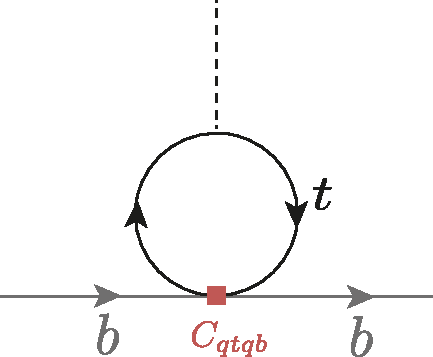
\includegraphics[width=0.8in]{./fig/cquqd_yuk}} &$ 2 N_c+1$ & $\CF$ & $y_t \, m_b\, m_t^2$ \vspace{0.2in} \\
			\hspace{-0.2in }\parbox[c]{1em}{
				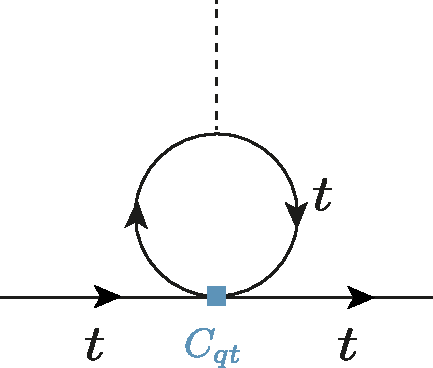
\includegraphics[width=0.8in]{./fig/cqt_yuk}} &1 & $\CF$ & $y_t \, m_t^3$ \vspace{0.2in} \\
			\hspace{-0.2in }\parbox[c]{1em}{
				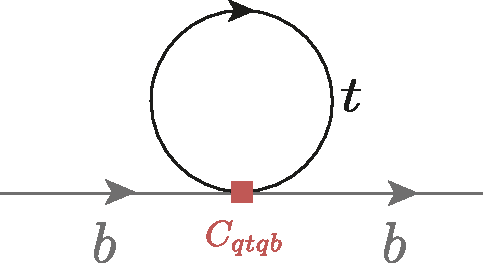
\includegraphics[width=0.8in]{./fig/self_cqtqb}} &$ 2 N_c+1$ & $\CF$ & $ m_t^3$ \vspace{0.2in} \\
			\hspace{-0.2in }\parbox[c]{1em}{
				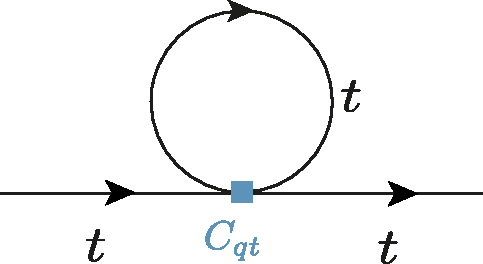
\includegraphics[width=0.8in]{./fig/self_cqt}} &$ 1$ & $\CF$ & $ m_t^3$ \vspace{0.2in} \\
			\midtopline
		\end{tabular}
		\caption{Sub-diagrams contributing to the NLO corrections of gluon fusion Higgs production and its decay to gluons, photons and beauty quarks.  }
		\label{tab:subdiagrams}
	\end{table}
	The effect of the beauty-quark loops coming from for~$ C_{QtQb}^{(1/8)}$ can be easily read from this table by exchanging~$ t \leftrightarrow b$. Although such corrections are significantly smaller than their counterparts coming from top-quark loops. 
	\par We see that these corrections correspond to the Wilson coefficients appearing in the RGE, and operators with (LL)(LL) or (RR(RR)) chiral structures do not contribute to these processes. \\ By considering the two-loop corrections to the ggF illustrated in~\autoref{fig:ggh} we find that such correction contains the sub-diagrams shown in~\autoref{tab:subdiagrams}, except for diagram (e), which is found to be vanishing for on-shell gluons. Additionally, these diagrams indicated that the two-loop corrections would be reduced to products of two one-loop functions after the integral reduction. \\
	Following the Feynman rules derived in ref.~\cite{Dedes:2017zog} for the four-fermion operators of interest here, the $ gg \to h$ two-loop amplitude was calculated, then Dirac algebra and further algebraic manipulations were preformed in Mathematica using~\texttt{PackageX}~\cite{Patel:2015tea}. Reduction of the resulting two-loop loop integrals to Master integrals has been preformed using~\texttt{KIRA}~\cite{Maierhoefer:2017hyi}. The computation has been cross-checked independently by my collaborators, using a different pipeline: \texttt{FeynArts}~\cite{Hahn:2000kx}, for amplitude generation then  \texttt{FeynRules}~\cite{Alloul:2013bka}  and  \texttt{Fire}~\cite{Smirnov:2008iw} for algebraic manipulation and loop-integral reduction. \\
	\par
	The sub-diagrams appearing in the two-loop calculation corresponds to mass and vertex renormalisation, which require counter-terms for pole cancellation. A mixture of an on-shell (OS) and $\MSbar$ -- schemes have been used for the mass and ~$h q \bar{q}$ coupling renormalisation, respectively. The renormalisation of SM quantities is  done in the OS scheme, while the NP parameters are renormalised according to the $\MSbar$ scheme. This method of mixed-scheme renormalisation was proposed by~\cite{Dawson:2018pyl}.
	\par The top/beauty mass renormalisation can be expressed as  
	\begin{equation}
		m_{t/b}^{\text{OS}}=m_{t/b}^{(0)}-\delta m_{t/b},
	\end{equation}
	with the corresponding counter-terms
	\begin{align}
		\delta m_t =&\frac{1}{8 \pi^2} \frac{C_{Qt}^{(1)}+c_F C_{Qt}^{(8)}}{\Lambda^2}m_t^3\left[ \frac{2}{\bar{\epsilon}} +2 \log\left(\frac{\mu_R^2}{m_t^2}\right)+1\right] \\ &- \frac{1}{16 \pi^2}  \frac{(2 N_c+1) C_{QtQb}^{(1)}+c_F C_{QtQb}^{(8)}}{\Lambda^2}  \left[ \frac{1}{\bar{\epsilon}} +  \log\left(\frac{\mu_R^2}{m_b^2}\right)+1 \right]  m_b^3\,, \nonumber \\
		\delta m_b=&-\frac{1}{16 \pi^2} \frac{(2 N_c+1)C_{QtQb}^{(1)}+c_F C_{QtQb}^{(8)}}{\Lambda^2}\left[ \frac{1}{\bar{\epsilon}} +\log\left( \frac{\mu_R^2}{m_t^2}\right)+1\right] m_t^3\,.
	\end{align}
	Here, we have $\bar{\epsilon}^{-1} = \epsilon^{-1}- \gamma_E +\log(4 \pi)$, in dimensional regularisation in $d=4-2\epsilon$ dimensions. 
	It is possible to convert from OS to the $\MSbar$ -- scheme for mass counter-terms via the following relations
	\begin{align}
		\delta m_t^{\bar{\text{MS}}} =&\frac{1}{8 \pi^2} \frac{C_{Qt}^{(1)}+c_F C_{Qt}^{(8)}}{\Lambda^2}m_t^3\frac{1}{\bar{\epsilon}}+ \frac{1}{16 \pi^2}  \frac{(2 N_c+1) C_{QtQb}^{(1)}+c_F C_{QtQb}^{(8)}}{\Lambda^2}   \frac{1}{\bar{\epsilon}}  m_b^3\,,  \\
		\delta m_b^{\bar{\text{MS}}}=&\frac{1}{16 \pi^2} \frac{(2 N_c+1)C_{QtQb}^{(1)}+c_F C_{QtQb}^{(8)}}{\Lambda^2}\frac{1}{\bar{\epsilon}} m_t^3\,.
	\end{align} 
	The effect of changing to the mass renormalisation scheme is small for the top quark but significant, up to $100\%$ effect, for the beauty. \\
	The top/beauty Higgs coupling in SMEFT, is written as
	\begin{equation}
		g_{ht\bar{t}/hb\bar{b}}=\frac{m_{t/b}}{v}-\frac{v^2}{\Lambda^2}\frac{C_{t\phi/b\phi}}{\sqrt{2}}\,.
	\end{equation}
	Hence, a modification of the Higgs couplings to beauty and top quarks is generated by operator mixing, even if $C_{t\phi/b\phi}$ are set to zero at $\Lambda$. From this, the $\MSbar$ counter-term should take the form 
	\begin{align}
		\delta	g_{ht\bar{t}/hb\bar{b}} &=  {m_{t/b}\over v} \delta{m_{t/b}} -{v^2 \delta{C_{t\phi/b\phi}}\over \sqrt{2} },
	\end{align}
	where $\delta{C_{t\phi/b\phi}}$ is directly read from the anomalous dimension, see ref.~\cite{Alonso:2013hga}
	\begin{figure}[h!]
		\begin{center}
			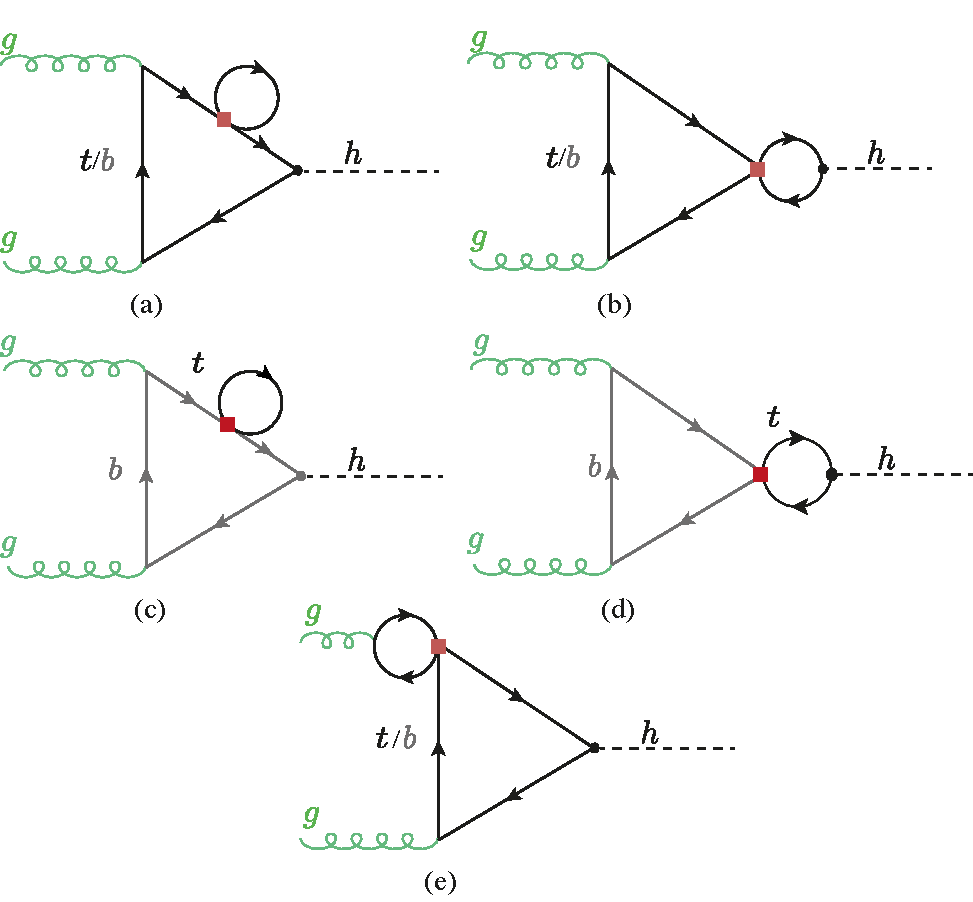
\includegraphics[width=8cm]{fig/ggF-4F_NLO.pdf}
			\caption{Example Feynman diagrams for the four-fermion-operator contributions to the Higgs production via gluon fusion. The red box indicates the four-fermion operator.\label{fig:ggh} }
		\end{center}
		\vspace{-1.5 cm}
	\end{figure}
	\begin{description}
		\item [\underline{Correction to gluon fusion and $h\to gg $ }] \hfill \vspace{0.3cm} \\
		The modification of the Higgs production via gluon fusion can be written as
		\begin{equation}
			\frac{\sigma_{ggF}}{\sigma_{ggF}^{\SM}}= 1+ \frac{ \sum_{i=t,b} 2 \Re(F_{\LO}^i F^*_{\NLO})}{\left| F_{\LO}^t+F_{\LO}^b  \right|^2}, \label{eq:production}
		\end{equation}
		with 
		%
		\begin{equation}
			F_{\LO}^i=-\frac{8m_i^2}{m_h^2}\left[1-\frac{1}{4}\log^2(x_i)\left(1-\frac{4m_i^2}{m_h^2}\right)\right],
		\end{equation}
		and the NLO form-factors are given by
		%
		\begin{equation}
			\begin{split}
				F_{\NLO}=&\frac{ 1}{4\pi^2  \Lambda^2}(C_{Qt}^{(1)}+c_FC_{Qt}^{(8)})F_{\LO}^t \left[ 2 m_t^2  +\frac{1}{4} (m_h^2-4 m_t^2) \left( 3 +2 \sqrt{1-\frac{4 m_t^2}{m_h^2}} \log(x_t) \right)  \right. \\ & \left.
				+\frac{1}{2} (m_h^2-4 m_t^2) \log\left(\frac{\mu_R^2}{m_t^2}\right)\right] \\ & + 
				\frac{1}{32 \pi^2 \Lambda^2} ((2N_c+1)C_{QtQb}^{(1)}+c_FC_{QtQb}^{(8)}) \left[ F_{\LO}^b \frac{m_t}{m_b}\left( 4 m_t^2-2 m_h^2 \right. \right.\\ & \left. \left. - (m_h^2-4 m_t^2)\sqrt{1-\frac{4 m_t^2}{m_h^2}} \log(x_t)-(m_h^2-4 m_t^2)\log\left(\frac{\mu_R^2}{m_t^2}\right)\right) +(t\leftrightarrow b)\right]  \,. \label{eq:FNLO}
			\end{split}
		\end{equation}
		Only top-quark loops contribute to the parts proportional to $C_{Qt}^{(1),(8)}$. 
		%
		The variable $x_i$ for a loop particle with mass $m_i$ is given by
		\begin{equation}
			x_i=\frac{-1+\sqrt{1-\frac{4 m_i^2}{m_h^2}}}{1+\sqrt{1-\frac{4 m_i^2}{m_h^2}}}\,. \label{eq:xvariable}
		\end{equation} 
		Using the same amplitudes, the~$ h \to gg$  partial width modification  can be written as
		\begin{equation}
			\frac{\Gamma_{h\to gg}}{\Gamma_{h\to gg}^{\SM}}= 1+ \frac{ \sum_{i=t,b} 2 \Re(F_{\LO}^i F^*_{\NLO})}{ |F_{\LO}^t+F_{\LO}^b|^2}.
		\end{equation}
		\item [\underline{Correction to Higgs decay to photons }] \hfill  \vspace{0.3cm} \\
	Since the decay~$ h \to \gamma \gamma$ contains the same topologies as gluon fusion, it is possible to use the results from the above calculation in obtaining the NLO correction to the partial width for this decay
		\begin{equation}
			\frac{\Gamma_{h\to \gamma\gamma}}{\Gamma_{h\to \gamma\gamma}^{\SM}}= 1+ \frac{2 \Re(F_{\LO, \gamma} F^*_{\NLO,\gamma})}{  |F_{\LO, \gamma}|^2} .
		\end{equation}
		However, one should pay attention to the change in the prefactors, and the extra EW contributions for~$ h \to \gamma \gamma$ 
		\begin{equation}
			F_{\LO, \gamma}= N_C\,Q_t^2 F_{\LO}^t+ N_C\,Q_b^2 F_{\LO}^b+F_{\LO}^W+ F^G_{LO} ,
		\end{equation}
		and $F_{\NLO, \gamma}$ is obtained from $F_{\NLO}$ by replacing the LO form-factor that appears inside of it by~$ F_{\LO}^i \to N_c \,Q_i^2 F_{\LO}^i$. The charges of the top and beauty quarks are $Q_t=2/3$ and $Q_b=-1/3$, respectively.\\ The $W$-boson loops contribution is given by
		%
		\begin{equation}
			F_{\LO}^W= 2 \left(1+6 \frac{m_W^2}{m_h^2}\right)-6 \frac{m_W^2}{  m_h^2} \left(1-2  \frac{m_W^2}{m_h^2}\right) \log^2(x_W),
		\end{equation}
		, and the Goldstone contribution
		%
		\begin{equation}
			F_{\LO}^G=4\frac{m_W^2}{m_h^2} \left( 1+ \frac{m_W^2}{m_h^2} \,\log^2(x_W) \right)\,.
		\end{equation}
		These operators also affect the $h\to Z\gamma$ partial width. However, as in the diphoton case, the effect is expected to be small due to the dominance of the $W$-boson contributions.  Furthermore, given the smallness of the $h\to Z\gamma$ branching ratio and the relatively low precision expected in probing this channel at the LHC, the effects of four-fermion interactions in the $ h \to Z\gamma$ decay are neglected in this study.
		\item [\underline{Correction to Higgs decays to $b \bar{b}$ }] \hfill  \vspace{0.3cm} \\
		The dominant four-fermion contributions to decay channel $h \to b\bar b$ come from the operators  $\mathcal{O}_{QtQb}^{(1),(8)}$; the corresponding diagram at NLO is shown in~fig~\ref{hbb}. 
		Adopting the same renormalisation procedure as described earlier, we have the following expression for the correction to 
		the $h \to b\bar b$ decay rate in the presence of ${\cal O}_{QtQb}^{(1),(8)}$
		\begin{equation}
			\begin{split}
				\frac{\Gamma_{h\to b\bar{b}}}{\Gamma_{h\to b\bar{b}}^{\SM}}=& 1+ \frac{1}{16\pi^2}\frac{m_t}{m_b}(m_h^2-4m_t^2)\frac{(2 N_c+1) C_{QtQb}^{(1)}+c_F C_{QtQb}^{(8)}}{\Lambda^2} \\ & \times\left[ 2+\sqrt{1-\frac{4 m_t^2}{m_h^2}}\log(x_t)-\log\left(\frac{m_t^2}{\mu_R^2}\right) \right] \,.
				\label{hbbnlo}
			\end{split}
		\end{equation}
		This NLO correction carries an enhancement factor of $m_t/m_b$ and is hence expected to be rather large.
	\end{description}
	\begin{figure}[h!]
		%\vspace{-.5 cm}
		\centering
		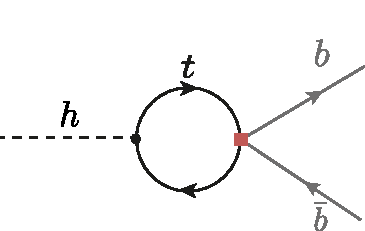
\includegraphics[scale=0.8]{./figures/Hbb}
		\caption{Feynman diagram contributing to the NLO   $h \to b \bar b$ process. }
		\label{hbb}
	\end{figure}
	The results of the NLO effects from the four-fermion operators reported above do not take into account the running of the Wilson coefficients. This would be based on assuming that these coefficients are defined at the process scale. Nevertheless, when we want to compare different processes or assume that the four-fermion operators are defined at the UV scale~$\Lambda$. One has to consider the running of these Wilson coefficients from~$\Lambda$ down to the process scale.\\
	These running effects can be included via the RGE for the operators with Wilson coefficient $C_{t\phi}$  and $C_{b\phi}$  \cite{Jenkins:2013zja, Jenkins:2013wua}, that leads approximatively to 
	\begin{equation}
		\begin{split}
			C_{t\phi}(\mu_R)-C_{t\phi}(\Lambda)= &\frac{1}{16 \pi^2 v^2} \left[-2  y_t (m_h^2  -4 m_t^2) (C_{Qt}^{(1)}+c_F C_{Qt}^{(8)} )\log\left( \frac{\mu_R^2}{\Lambda^2}\right) \right.\\
			& \left.+ \frac{y_b}{2} (m_h^2-4 m_b^2)\left(  (2N_c+1)  C_{QtQb}^{(1)}+   c_F C_{QtQb}^{(8)}\right)\log\left( \frac{\mu_R^2}{\Lambda^2}\right)\right], \label{eq:runningCuH}
		\end{split}
	\end{equation}
	and
	\begin{equation}
		\begin{split}
			C_{b\phi}(\mu_R)-C_{b\phi}(\Lambda)= \frac{y_t}{32 \pi^2 v^2} \left[  (m_h^2-4 m_t^2)\left(  (2N_c+1)  C_{QtQb}^{(1)}+   c_F C_{QtQb}^{(8)}\right)\log\left( \frac{\mu_R^2}{\Lambda^2}\right)\right]\,, \label{eq:runningCdH}
		\end{split}
	\end{equation}
	where $y_{t/b}=\sqrt{2} m_{t/b}/v$.
	Note that the combinations of the Wilson coefficients appearing in \eqref{eq:runningCuH} and \eqref{eq:runningCdH} are the same as in $F_{NLO}$ in \eqref{eq:FNLO}.
	Effectively, it is possible to obtain the result under the assumption that the four-fermion operators are the only non-zero ones at the large scale by replacing in \eqref{eq:FNLO} $\mu_R \to \Lambda$. Here the  op and beauty quark masses were renormalised the OS scheme.
	Including the leading logarithmic running of $C_{b\phi}$ of \eqref{eq:runningCdH} from the high scale $\Lambda$ to the electroweak scale is achieved by setting in \eqref{hbbnlo} $\mu_R\to \Lambda$.
	The expression in \eqref{hbbnlo} agrees with results obtained from the full calculation of the NLO effects in the dimension-six SMEFT, computed in ref.~\cite{Gauld:2015lmb}. 
	%%%%%%%%%%%%%%%%%%%%%%%%%%%%%%%%%%%%%%%%%%%%%%%%%%%%%%%%%%%%%%%%%%%%%
	\subsection{SMEFT-NLO calculation of  $t\bar th$}
	\begin{figure}[h!]
		\centering
		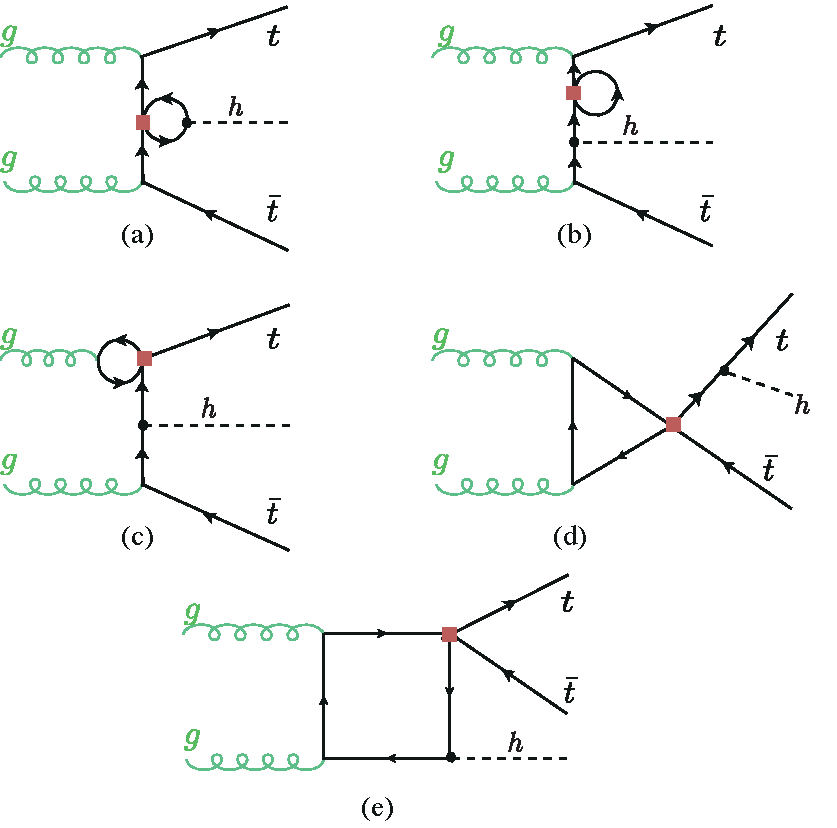
\includegraphics[width=8cm]{./fig/ggttH-4F_NLO}
		\caption{Feynman diagrams including the four-fermion loop contributions to the $ gg \to t\bar{t} h$ subprocess.}
		\label{ggtth}
	\end{figure}
	\begin{figure}[hth]
		\centering
		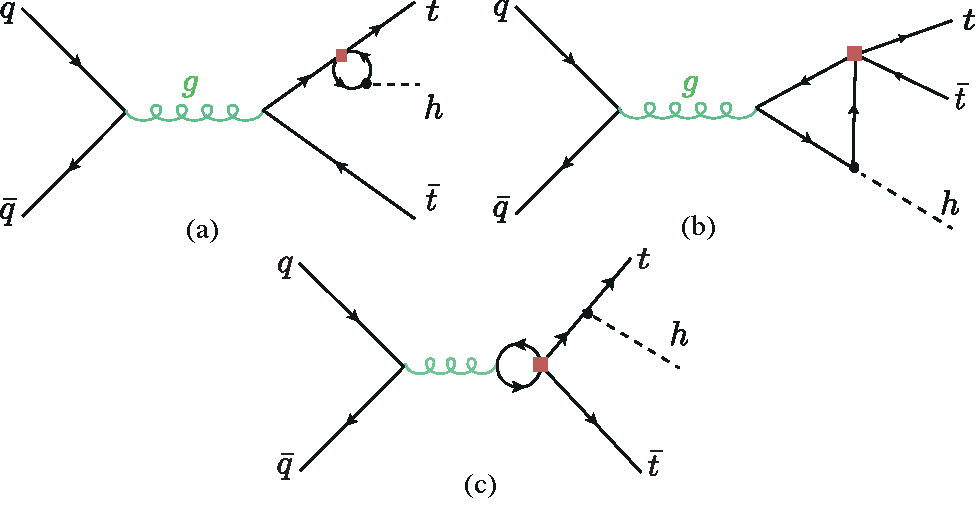
\includegraphics[width=8cm]{./fig/qqttH-4F_NLO}
		\caption{Feynman diagrams including the four-fermion loop contributions to the~$ q \bar{q} \to t\bar{t} h$ subprocess.}
		\label{qqtth}
	\end{figure}
	\par Unlike the previous processes, the associated production of the Higgs with top quark pair involves new topologies that are not limited to Yukawa vertex correction or mass renormalisation.  At the LHC, there are two sub-processes responsible for the~$t\bar t h$ production: gluon-initiated process that is depicted in~\autoref{ggtth} and quark-initiated that is seen  in~\autoref{qqtth}. The new \emph{finite} topologies induced by the four-fermion operator correction are: triangle and box topologies, shown in diagrams (d) and (e) in~\autoref{ggtth}, as well as in the triangle topology shown in diagram (b)  of~\autoref{qqtth}.  Additionally, the $t\bar t g$ vertex correction in the quark-initiated process~(diagram (c)) of~\autoref{qqtth} is non-vanishing as the gluon is off-shell. This vertex correction has a UV pole that requires a counter-term for its cancellation
	\begin{equation}
		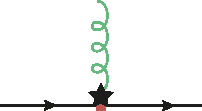
\includegraphics[width=0.13\linewidth]{fig/CT} =\frac{ig_s}{12 \pi^2\Lambda^2} T^{A}_{ij} p_g^2 \gamma^\mu \left( C_{tt} P_R+\left(C_{QQ}^{(1)} + C_{QQ}^{(3)}\right) P_L +\frac{ C_{Qt}^{(8)}}{4} \right) \left( \frac{1}{\bar{\epsilon}}-1 \right) . \label{eq:R2CT}
	\end{equation}
	Another difference between $t\bar t h$ and the other Higgs processes studied in this chapter is that this channel has a non-trivial colour structure. This manifests in the presence of multiple colour projectors, because the quark anti-quark triplets or the gluon pairs do not have to recombine to only a singlet state rather to both a singlet and an octet,  according to the expansion of product $ \irrep{3} \otimes \irrepbar{3}\to\irrep{1}+\irrep{8}$. This breaks the degeneracy between the singlet and octet Wilson coefficients. Lastly, due to the new topologies and  $t\bar t g$ vertex correction, operators with single chirality will contribute to NLO corrections, namely the operators $\mathcal O_{tt}$ and $\mathcal O_{QQ}^{(1,3)}$.\\
	%
	All of the four-fermion operators are implemented in the loop-capable UFO model \texttt{SMEFTatNLO}~\cite{Degrande:2020evl} that is computed via  \texttt{Madgraph\_aMCNLO} \cite{Alwall:2014hca} with some tweaking to remove the NLO QCD corrections. This is done via a user-defined loop filter function in Madgraph. The results were reproduced by an analytic computation based on the reduction of one-loop amplitudes via the method developed by G. Ossola, C.G. Papadopoulos and R. Pittau~(OPP reduction)~\cite{Ossola:2006us}, implemented in the FORTRAN code~\texttt{CutTools}~\cite{Ossola:2007ax}.
	This programme takes the full one-loop amplitude and then reduces it to terms with 1,2,3, and 4-point loop functions in four dimensions, keeping spurious terms from the $\epsilon$ part of the amplitude. To correct for such terms, one needs to compute the divergent UV counter-terms as well as finite rational terms, denoted by $R_{2}$ as in ref.~\cite{Ossola:2008xq}.\footnote{Another rational term~$R_1$ appears due to a mismatch between the four and $d$ dimensional amplitudes, but this is computed automatically in \texttt{CutTools}. } The amplitudes were generated in the same way as for ggF. The UV and $R_2$ counter-terms, which need to be supplemented to \texttt{CutTools}, were computed manually following the method detailed in~\cite{Ossola:2008xq}. For both codes, the  NNPDF23 PDF set at NLO \cite{Ball:2012cx} was used. 
	%
	\par The singlet and octet operators $\mathcal{O}_{QtQb}^{(1),(8)}$  contribute to $t \bar{t} h$ only via beauty-quark loops and, in principle, could be directly dismissed like the other beauty quark operators mentioned above. However, it is instructive to investigate their effect, albeit it is very small.
	Since the \texttt{SMEFTatNLO} model does not have these operators, it was needed to implement them manually in that model. This is simply done by including the vertices generated by these operators and their UV and $R_2$ counter-terms. The calculation of the NLO correction by these operators was done both in Madgraph using a modified UFO model and with the code based on  \texttt{CutTools}. The effects where comparable to the leading log effects computed using ~\texttt{SMEFTsim} package ~\cite{Brivio:2017btx} of $ \sim 10^{-6}$. Hence confirming the expectation that beauty quark loops have a negligible effect. 
	%
	\par To include the effects of Wilson coefficients' running, the relevant contribution for the gluon-initiated process is the same as the stated for the gluon fusion in~\eqref{eq:runningCuH}. While for the quark-initiated process, one needs to consider the operator mixing in the running, particularly between operators that contain second and third-generation quarks mixed. These corrections can be obtained from the RGEs in refs.~\cite{Jenkins:2013zja,Jenkins:2013wua, Alonso:2013hga}.
	%%%%%%%%%%%%%%%%%%%%%%%%%%%%%%%%%%%%%%%%%%%%%%%%%%%%%%%%%%%%%%%%%%%%%
	\subsection{Results}
	The NLO effects generated by the SMEFT four-fermion operators of the third generation quarks on the Higgs rate have been extracted from the above computation using the formula
	\begin{equation}
		\delta R(C_i) = R/R^{\SM} -1,
		\label{eq:deltaR}
	\end{equation}
	here the rates could either be cross-section $\sigma$ or partial width $\gamma$. The dependence of a given Higgs rate~$R$ on the Wilson coefficient $C_i$ is denoted by $\delta R(C_i) $.  Only contributions linear in the Wilson coefficients are considered. In order to isolate the finite terms from the ones coming from the RGE leading log approximation, the correction is further expanded to finite ~$\delta R_{C_i}^{fin}$ and leading log terms~$\delta R_{C_i}^{log}$ as follows
	\begin{equation}
		\delta R(C_i)= \frac{C_i}{\Lambda^2}\left(\delta R_{C_i}^{fin}+ \delta R_{C_i}^{log} \log\left(\frac{\mu_R^2}{\Lambda^2}\right)\right)\,.
		\label{eq:deltar}
	\end{equation}
	%
	Using this formula, one can obtain the correction at any NP scale $\Lambda$. Though, in the remainder of this chapter, this scale is set to \SI{1}{TeV}. In~\autoref{table:res4top}, the finite and logarithmic corrections for the operators considered in this study are reported. Using this table in filling the formula~\eqref{eq:deltar} gives the correction to the Higgs rate in question.  However, since some of the rates are Higgs partial widths, the Higgs total width~$\Gamma_h$ will be affected, and therefore, all Higgs rates are changed, as the branching fractions will carry the full width dependence on the Wilson coefficients.
	%
	An important observation from~\autoref{table:res4top} is that the finite terms, are either larger or at the same order than the leading-log ones, except for $h\to b\bar{b}$ corrections from~$C_{QtQb}^{(1),(8)}$. This highlights the importance of the full NLO calculation for these corrections in constraining these four-fermion operators, in particular~$\mathcal O_{Qt}^{(1),(8)}$.
	
\begin{table}[t!]
	\centering
	\small{
		\begin{tabular}{c||cccc}
			\toprule
			{ \normalsize Operator} &  { \normalsize Process }& { \normalsize $\mu_R$} & { \normalsize$ \delta R_{C_i}^{fin}\; [\text{TeV}^2]$} &{ \normalsize$ \delta R_{C_i}^{log}\; [\text{TeV}^2] $} \\
			\midrule
            \multirow{5}{*}{ { \normalsize$\mathcal{O}_{Qt}^{(1)}$}}  &  ggF& $\frac{m_h}{ 2}$&$\phantom{+}9.91\cdot 10^{-3}$&$\phantom{+}2.76\cdot 10^{-3}$\\     % \cmidrule(r){2-5}  
                                                                    &  $h \to gg$& \mr{$m_h$}&$\phantom{+}6.08\cdot 10^{-3}$&$\phantom{+}2.76\cdot 10^{-3}$\\
            	                                                   &  $h \to \gamma \gamma$& &$-1.76\cdot 10^{-3}$ &$-0.80\cdot 10^{-3}$ \\
            	                                              %     \cmidrule(r){2-5}    
            	                                                   	&  $t\bar t h$ {\color{Mahogany}  13 TeV }&\mr{ $m_t+\frac{m_h}{ 2}$}&$-4.20\cdot 10^{-1} $&$-2.78\cdot 10^{-3}$\\	    
            	                                                   	&   $t\bar t h$  {\color{Mahogany}  14 TeV }& &$-4.30\cdot 10^{-1} $&  $-2.78\cdot 10^{-3}$\\	
            	                                                   	\midrule
          \multirow{5}{*}{ { \normalsize$\mathcal{O}_{Qt}^{(8)}$} } & ggF& {$\frac{m_h}{ 2}$}&$\phantom{+}1.32\cdot 10^{-2}$&$\phantom{+}3.68\cdot 10^{-3}$\\    %  \cmidrule(r){2-5}  
                                                                   &  $h \to gg$& \mr{$m_h$}&$\phantom{+}8.11\cdot 10^{-3}$&$\phantom{+}3.68\cdot 10^{-3}$\\
            	                                                   	&  $h \to \gamma \gamma$& &$-2.09\cdot 10^{-3}$&$-1.07\cdot 10^{-3}$\\
            	                                                   %	 \cmidrule(r){2-5}    
            	                                                   	&  $t\bar t h$ {\color{Mahogany}  13 TeV }& \mr{$m_t+\frac{m_h}{ 2}$}&$\phantom{+}6.81\cdot 10^{-2}$ &$-2.40\cdot 10^{-3}$\\	    
            	                                                   	&   $t\bar t h$  {\color{Mahogany}  14 TeV }& & $\phantom{+}7.29\cdot 10^{-2}$&  $-2.48\cdot 10^{-3}$\\	              
                       	                                                   	\midrule
           \multirow{4}{*}{ { \normalsize$\mathcal{O}_{QtQb}^{(1)}$} } & ggF& ${m_h\over 2}$&$\phantom{+}2.84\cdot 10^{-2}$&$\phantom{+}9.21\cdot 10^{-3}$\\   %   \cmidrule(r){2-5}  
            &  $h \to gg$& \multirow{3}{*}{$m_h$}&$\phantom{+}1.57\cdot 10^{-2}$&$\phantom{+}9.21\cdot 10^{-3}$\\
           &  $h \to \gamma \gamma$& &$-1.30\cdot 10^{-3}$&$-0.78\cdot 10^{-3}$\\
           &  $h \to b \bar b$& &$\phantom{+}9.25\cdot 10^{-2}$&$\phantom{+}1.68\cdot 10^{-1}$\\
         %   \cmidrule(r){2-5}    
			\midrule
			 \multirow{4}{*}{{ \normalsize$\mathcal{O}_{QtQb}^{(8)}$}}  & ggF& {$\frac{m_h}{ 2}$}&$\phantom{+}5.41\cdot 10^{-3}$&$\phantom{+}1.76\cdot 10^{-3}$\\      %\cmidrule(r){2-5}  
			 & $h \to gg$& \multirow{3}{*}{$m_h$}&$\phantom{+}2.98\cdot 10^{-3}$&$\phantom{+}1.76\cdot 10^{-3}$\\
			&  $h \to \gamma \gamma$& &$-0.25\cdot 10^{-3}$& $-0.15\cdot 10^{-3}$\\
			&  $h \to b \bar b$& &$\phantom{+}1.76\cdot 10^{-2}$&$\phantom{+}3.20\cdot 10^{-2}$\\
			% \cmidrule(r){2-5}    
			\midrule	    	 
			 \multirow{2}{*}{{ \normalsize$\mathcal{O}_{QQ}^{(1)}$}  }
			 	&  $t\bar t h$ {\color{Mahogany}  13 TeV }& \mr{$m_t+\frac{m_h}{ 2}$}&  {$\phantom{+}1.75\cdot 10^{-3}$} &$\phantom{+}1.84\cdot 10^{-3}$\\	    
			 &   $t\bar t h$  {\color{Mahogany}  14 TeV }& & $\phantom{+}1.65\cdot 10^{-3}$& $\phantom{+}1.76\cdot 10^{-3}$\\          
			 \midrule	    	 
			 \multirow{2}{*}{{ \normalsize$\mathcal{O}_{QQ}^{(3)}$}  }
			 &  $t\bar t h$ {\color{Mahogany}  13 TeV }& \mr{$m_t+\frac{m_h}{ 2}$}&  $\phantom{+}1.32\cdot 10^{-2}$ & $\phantom{+}5.48\cdot 10^{-3}$\\	    
			 &   $t\bar t h$  {\color{Mahogany}  14 TeV }& & $\phantom{+}1.24\cdot 10^{-2}$& $\phantom{+}5.30\cdot 10^{-3}$\\        
			  \midrule	    	 
			 \multirow{2}{*}{{ \normalsize$\mathcal{O}_{tt}$}  }
			 &  $t\bar t h$ {\color{Mahogany}  13 TeV }& \mr{$m_t+\frac{m_h}{ 2}$}&  $\phantom{+}4.60\cdot 10^{-3}$ &$\phantom{+}1.82\cdot 10^{-3}$\\	    
			 &   $t\bar t h$  {\color{Mahogany}  14 TeV }& & $\phantom{+}4.57\cdot 10^{-3}$& $\phantom{+}1.74\cdot 10^{-3}$\\                                           	
			\bottomrule
		\end{tabular}
	}
\caption{The NLO effects of the four heavy-quarks operators on the Higgs rates. The effects are separated into finite ~$ \delta R_{C_i}^{fin}$ and leading log~ parts, in correspondence with~\eqref{eq:deltar}.  This table has been published in~\cite{Alasfar:2022zyr}.}
\label{table:res4top}
\end{table}


	%The numerical values were obtained using as input parameters
	%\begin{equation}
	%	\begin{split}
		%		& G_F=1.166378 \cdot 10^{-5} \text{ GeV}^{-2}\,,  \; m_W=80.379\text{ GeV}\,, \;m_Z=91.1876\text{ GeV}\,, \\ &  m_t^{\text{OS}}=172.5 \text{ GeV}\,, \; m_b^{\text{OS}}=4.7\text{ GeV}\,,  \;m_h=125.1\text{ GeV}\,,
		%	\end{split}
	%\end{equation}
	\par As mentioned earlier, there is a degeneracy between the singlet and octet operators, seen clearly in the analytic result for gluon fusion and the Higgs decays considered. This degeneracy is though broken for~$\mathcal O_{Qt}^{(1),(8)}$ due to $t\bar t h$. Since, the effect of ~$\mathcal O_{QtQb}^{(1),(8)}$ is negligible for this process, the independent degree of freedom for these operators' Wilson coefficients is the linear combination
	\begin{equation}
		C_{QtQb}^+= (2N_c+1 )C_{QtQb}^{(1)} + c_F   C_{QtQb}^{(8)}.
		\label{eq:CQtQbplus}
	\end{equation}
	%
	%%%%%%%%%%%%%%%%%%%
	\section{Fit to Higgs observables \label{sec:fit}}
	%%%%%%%%%%%%%%%%%%%
	
	\par Using the results from the  NLO calculations discussed above and combining them with the calculations of NLO Higgs rates from the trilinear Higgs self-coupling~$\lambda_3$, performed in refs.~\cite{Gorbahn:2016uoy, Degrassi:2016wml, Bizon:2016wgr, Maltoni:2017ims, Degrassi:2021uik}, the previous fits on $\lambda_3$ from single-Higgs observables can be extended with the inclusion of these four-fermion SMEFT Wilson coefficients. Hence, we revisit the sensitivity studies of single Higgs observables to the trilinear coupling~$\lambda_3$.  
	Although combined fits from Higgs data, including $\lambda_3$ and SMEFT operators modifying Higgs rates at LO, have been preformed already, e.g. in ref.~\cite{DiVita:2017eyz}. Such fits would not be sufficient to determine the actual sensitivity for $\lambda_3$. In particular, if the SMEFT operators are weakly constrained and induce significant modifications to Higgs rates, which can be seen in~\autoref{table:res4top}. This chapter does not include a global SMEFT fit; instead merely motivates it by illustrating how the sensitivity for probing the Higgs-self coupling from single Higgs data gets mitigated when the four-fermion operators are included in the fit.
	%
	\par In the antecedent studies, the modification to Higgs self coupling was reported in terms of the $\kappa$-formalism, for the consistency of this analysis, the NLO corrections from the trilinear self-coupling will be converted to the SMEFT notation, in terms of the Wilson coefficient~$C_\phi$, for more details on the conversion between SMEFT and $\kappa$-formalism see~\autoref{eftkappa}. In order to keep track of he SMEFT power-counting, the results of ~\cite{Degrassi:2016wml} are rewritten in terms of the SMEFT Wilson coefficient $C_\phi$
	\begin{equation}
		\delta R_{\lambda_3}\equiv\frac{R_\mathrm{ NLO}(\lambda_3)-R_\mathrm{ NLO}(\lambda_3^\mathrm{{SM}})}{R_\mathrm{ LO}}=-2\frac{C_{\phi}v^4}{\Lambda^2 m_h^2}C_1 + \left(-4\frac{C_{\phi}v^4}{\Lambda^2 m_h^2}+4\frac{C_{\phi}^2 v^8}{m_h^4\Lambda^4}\right) C_2 . \;\;\;\;\;
		\label{eq:degrassi}
	\end{equation}
	%
	In \eqref{eq:degrassi}, the coefficient $C_1$ corresponds to the contribution of the trilinear coupling to the single Higgs processes at one loop, adopting the same notation as~\cite{Degrassi:2016wml}. The values of $C_1$ for the different processes of interest for this study are given in~\autoref{table:resch}. The coefficient $C_2$ describes universal corrections and is given by
	\begin{equation}
		C_2=\frac{\delta Z_h}{1-\left(1-\frac{2 C_\phi v^4}{\Lambda^2 m_h^2}\right)^2 \delta Z_h}\,, \label{eq:C2}
	\end{equation}
	%
	where the constant $\delta Z_h$ is the SM contribution from the Higgs loops to the wave function renormalisation of the Higgs boson,
	\begin{equation}
		\delta Z_h =-\frac{9}{16}\,\frac{G_F m_h^2}{\sqrt{2}\pi^2}\left(\frac{2\pi}{3\sqrt{3}}-1\right).
	\end{equation}
	The coefficient $C_2$ thus introduces additional $\mathcal{O}(1/\Lambda^4)$ (and higher order) terms in $\delta R_{\lambda_3}$.  
	In ref.~\cite{Degrassi:2016wml} considering the $\kappa$-formalism, the full expression of \eqref{eq:C2} is kept, while having two different descriptions: one in which $\delta R_{\lambda_3}$ is expanded up to linear order in $C_\phi$ and an alternative scheme in which terms up to $\mathcal{O}(1/\Lambda^4)$ are also kept in the EFT expansion. Keeping the full expression in \eqref{eq:C2} and including terms up to $\mathcal{O}(1/\Lambda^4)$  in $C_2$ lead to nearly the same results as the simple~$\mathcal{O}(1/\Lambda^4)$ fit.
	%{ \footnotesize
\begin{table}[h]
\centering
\begin{tabular}{lr}
\toprule
Process&$C_1\cdot 10^{-2}$,  $(\Lambda=1 \mathrm{TeV} )$  \\
\midrule
ggF/ $gg\to h$   & -0.31 \\
$t\bar{t}h$   \textcolor{Mahogany}{13 TeV}   & -1.64 \\
$t\bar{t}h$   \textcolor{Mahogany}{14 TeV}   & -1.62 \\
$h\to \gamma \gamma$   & -0.23 \\
$h\to b\bar{b}$ & 0.00  \\
$h\to W^+ W^-$  & -0.34 \\
$h\to Z Z$      & -0.39 \\
$pp\to Zh$   \textcolor{Mahogany}{13 TeV}    & -0.56 \\
$pp\to Zh$    \textcolor{Mahogany}{14 TeV}    & -0.55 \\
$pp\to W^\pm h$  & -0.48 \\
VBF              & -0.30 \\
$ h \to 4 \ell$              & -0.38 \\
\bottomrule
\end{tabular}
\caption{The relative correction dependence on $C_\phi$ for single Higgs processes taken from~\cite{ Degrassi:2021uik}. If the $\sqrt{s}$ is not indicated, the $C_1$ coefficient (see eq.~\eqref{eq:degrassi}) is the same for both $13$ and $14$ TeV. \la{I suggest we remove this, as we do not use these number in the fit -.. the aim of this is to comparew tih 4F, but it maybe confusing}}
\label{table:resch}
\end{table}
%}
	%
	A Bayesian fit was preformed using Markov-chain Monte Carlo~(MCMC) method.   Using a flat prior s~$ \pi(C_i)= const.$ and a log likelihood of a Gaussian distribution 
	\begin{equation}
		\log(L) = -\frac{1}{2}\left[  (\vec{\mu}_{\mathrm{Exp}} -\vec{\mu} ) ^{T} \cdot \mathbf{V}^{-1} \cdot ( \vec{\mu}_{\mathrm{Exp}} -\vec{\mu} )\right]  .
		\label{eq:loglike}
	\end{equation}
	Constructed as follows:
	\begin{description}
		\item[Experimental inputs $\vec{\mu}_{\mathrm{Exp}}$ ] The signal strengths from experimental measurements of single Higgs rates defined as
		\begin{equation}
			\mu_{\mathrm{Exp}}\equiv \sigma_{\mathrm{obs}}/\sigma_\SM.
		\end{equation}
		These measurements as taken from LHC Run II for centre-of-mass energy of $\sqrt{s} = 13$ TeV and  integrated luminosity of $ 139\, \mathrm{fb}^{-1}$ for ATLAS and  $ 137\,\mathrm{fb}^{-1}$ for CMS. In addition to HL-LHC projections by CMS for $\sqrt{s} = 14$ TeV and integrated luminosity of $ 3000\, \mathrm{fb}^{-1}$. Both of these inputs have been already discussed in~\autoref{chap:HiggsConstr} and summarised in~\autoref{table:resHiggsExp}.
		\item [Theoretical predictions $\vec{\mu}$ ]  The corresponding theoretical predictions for each of the experimental measurement /projections have been built using the modification to the cross-sections and branching ratios coming from the SMEFT four-fermion operators and $C_\phi$. To keep with the power-counting, the signal strength is also expanded in powers of $\Lambda$, keeping only $ \Lambda^{-2}$ terms. 
		\begin{equation}
			\mu(C_\phi,C_i)=\frac{\sigma_\mathrm{ Prod}(C_\phi,C_i) \times \mathrm{ BR}(C_\phi,C_i)}{\sigma_\mathrm{ Prod, SM}\times \mathrm{BR}_\mathrm{ SM}} \approx 1+\delta \sigma(C_\phi,C_i)+\delta\Gamma(C_\phi,C_i)-\delta \Gamma_h(C_\phi,C_i).
			\label{linear-mu}
		\end{equation}
		\item [Uncertainties and correlations $\mathbf{V}$ ]  The variance matrix~$\mathbf{V}$ is build from thee experimental uncertainties found in ~\autoref{table:resHiggsExp}. For Run-II data, only ATLAS collaboration reported the correlation amongst different channels of which only correlations $> 10\%$ are considered, while for the HL-LHC, the whole correlation matrix found on the webpage~\cite{twiki}.  The HL-LHC projections for the S2 scenario explained in~\cite{Cepeda:2019klc} were used. These assume the improvement on the systematics that is expected to be attained by the end of the HL-LHC physics programme, and that theory uncertainties are improved by a factor of two with respect to current values. Theoretical uncertainties were not considered in this fit.
	\end{description}
	The python package~\texttt{pymc3}~\cite{Salvatier2016} was used to construct the posterior distribution. I have used the \texttt{Arviz} Bayesian analysis package~\cite{arviz_2019} to extract the credible intervals (CIs) from the highest density posterior intervals~(HDPI) of the posterior distributions, where the intervals covering 95\% (68\%) of the posterior distribution are considered the 95\% (68\%) CIs. In the Gaussian limit, these  95\% (68\%) CIs should be interpreted as equivalent to the 95\%  (68\%) Frequentist  confidence level~(CL) two-sided bounds. \HEPfit~\cite{deBlas:2019okz} code was used to validate the fits.
	%%%%
	Given that current bounds on these operators are rather weak, one may wonder about the uncertainty in these fits associated with the truncation of the EFT.
	Note that, since the four-quark operators only enter into the virtual corrections at NLO, Higgs production and decay contain only linear terms in $1/\Lambda^{2}$ in the corresponding Wilson coefficients, i.e.~the quadratic terms coming from squaring the amplitudes are technically NNLO. 
	Hence, the quadratic effects in the signal strengths coming from not linearising the corrections to the product $\sigma_\mathrm{ Prod} \times \mathrm{ BR}$~\!.  These effects have been investigated and found to have a negligible impact on the fit. 
	The operators of single chirality~$\mathcal O_{tt}$ and $\mathcal{O}_{QQ}^{(1)/(3)}$ were not included in the fit, as their effect on Higgs rates is limited to small $\delta R$ for $t\bar t h$. Thus, they cannot be contained simultaneously with $C_\phi$ using single Higgs data.  
	\subsection{Fit results}
	\par 
	In~\autoref{2param-cqt} and~\autoref{2param-cqtqb}, I show the $68\%$ and $ 95\%$  CIs of the two-parameter posterior distributions and their marginalisation for the two-parameter fits involving $C_\phi$ and one of the four-heavy quark Wilson coefficients, evaluated at the scale $\Lambda=1$ TeV for Run-II LHC measurements.  
	Both linearised and quadratically truncated $\delta R_{\lambda_3}$ fits are shown, and one can observe that the $95\%$ CI bounds (shown on top of the panels) and correlations depend on the truncation.
	\begin{figure}[h!]
		\begin{center}
			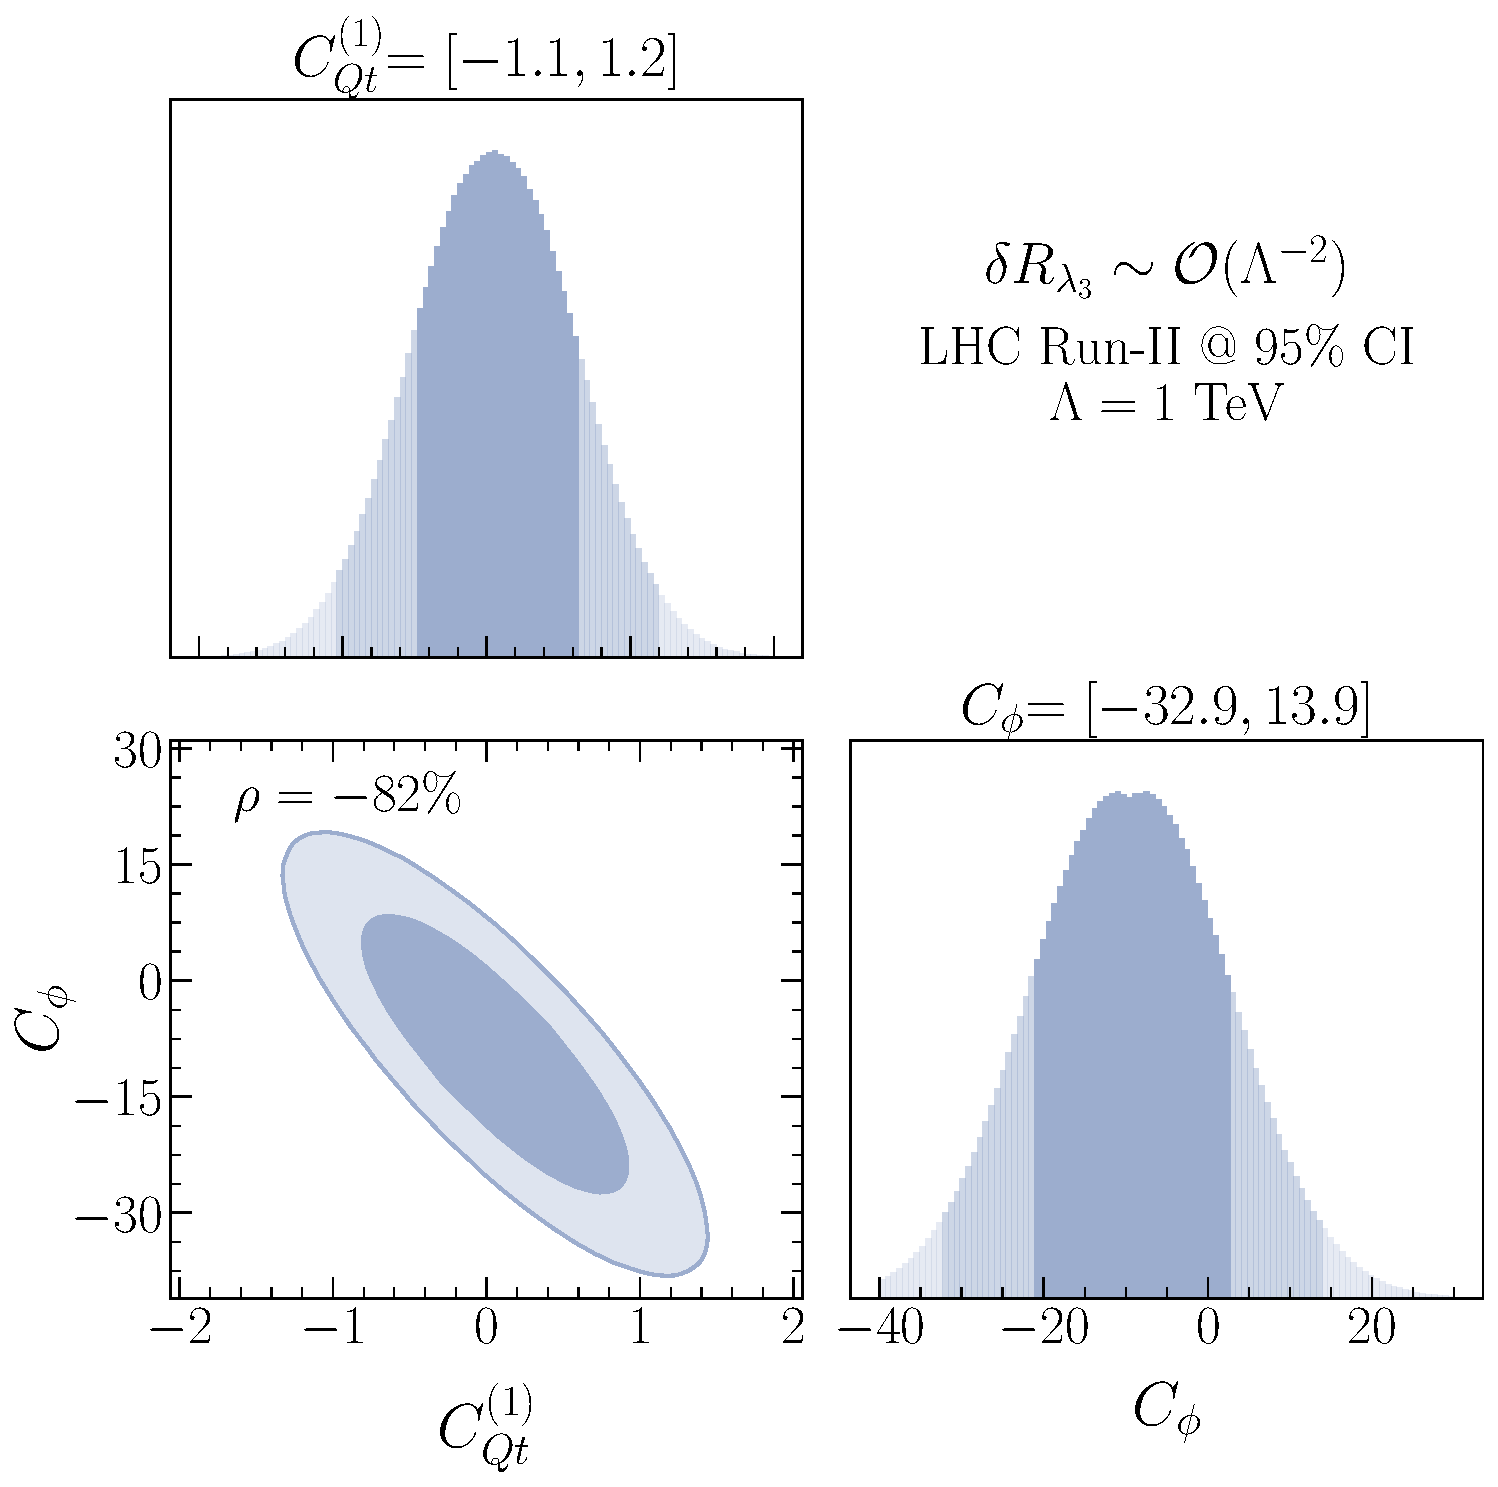
\includegraphics[width=0.45\linewidth]{fig/Cqt1_LHC_RunII_linearl3_rge}
			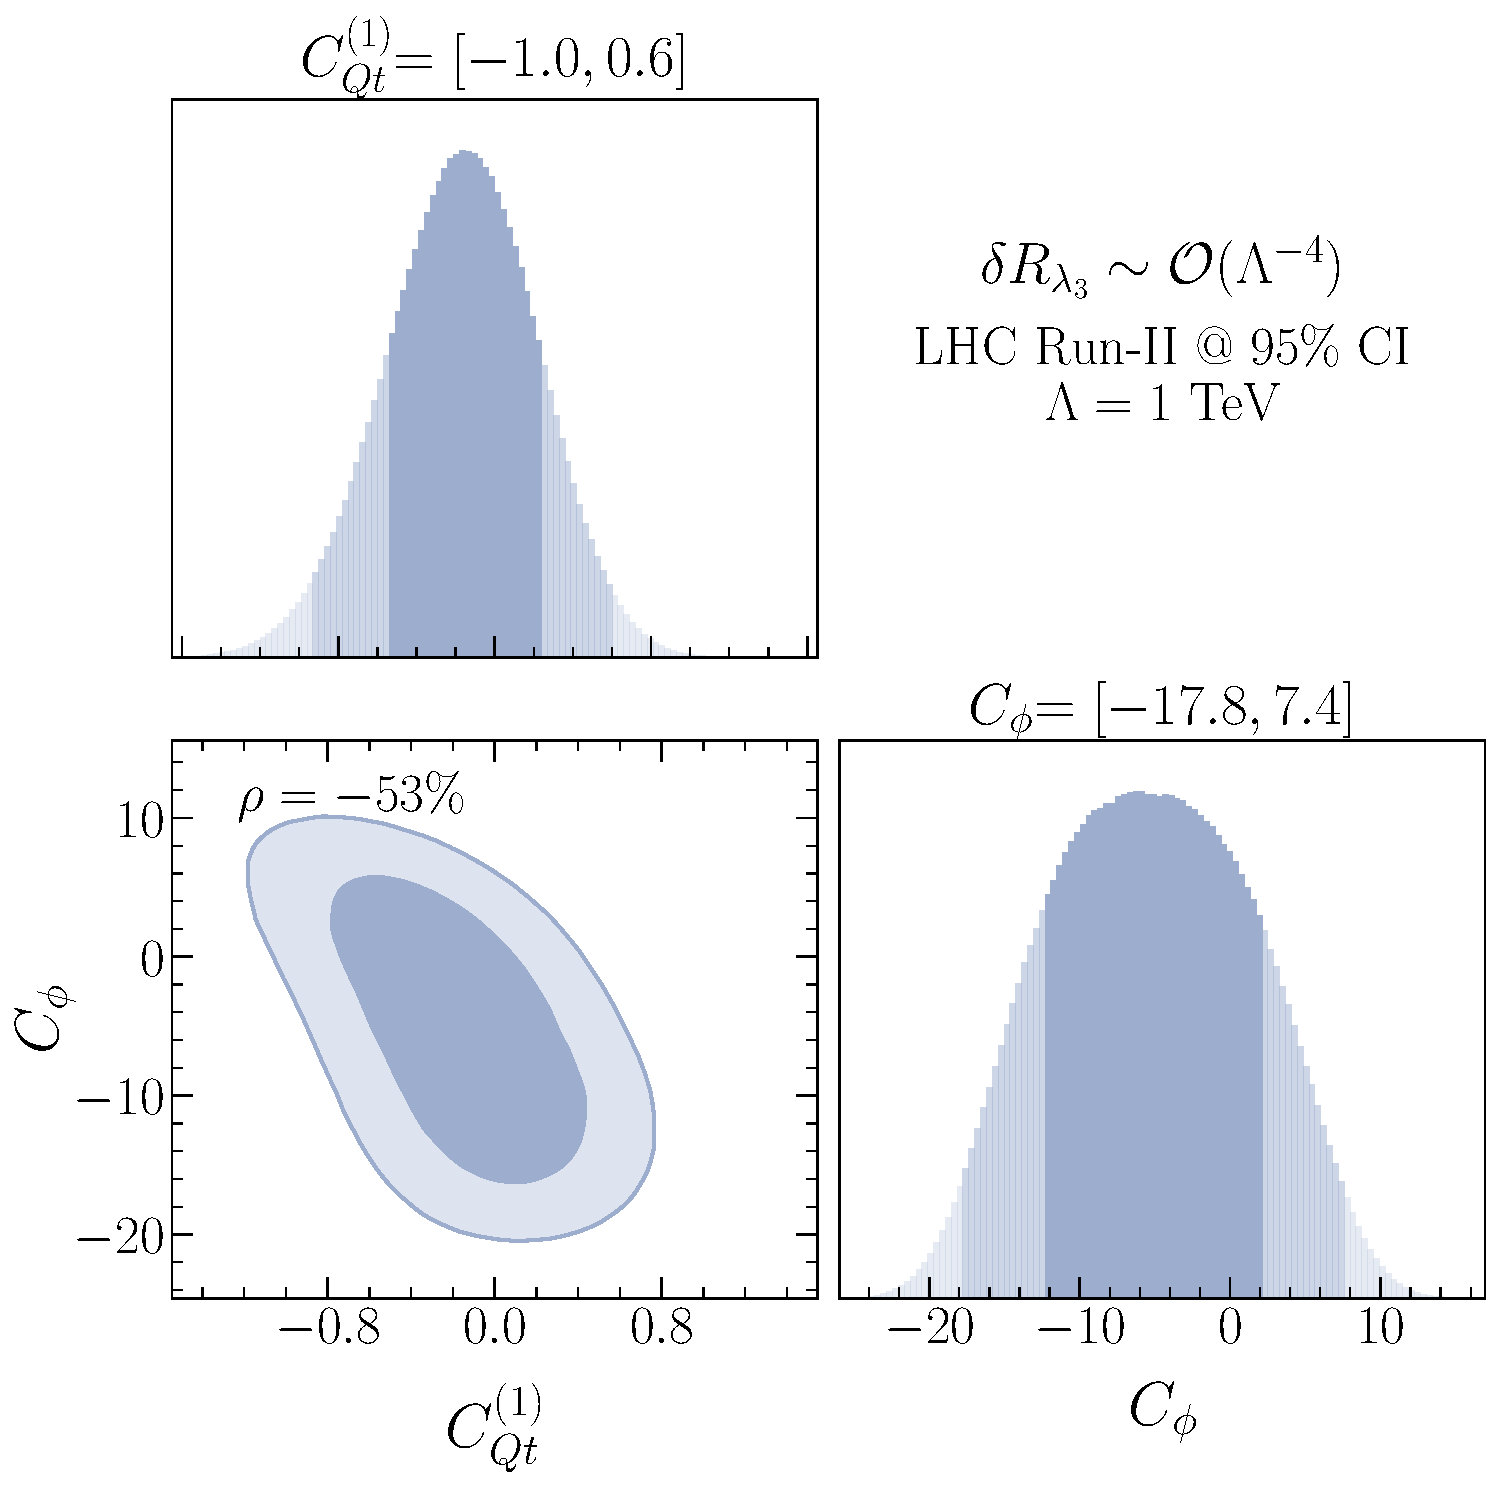
\includegraphics[width=0.45\linewidth]{fig/Cqt1_LHC_RunII_quadl3_rge} \\ 
			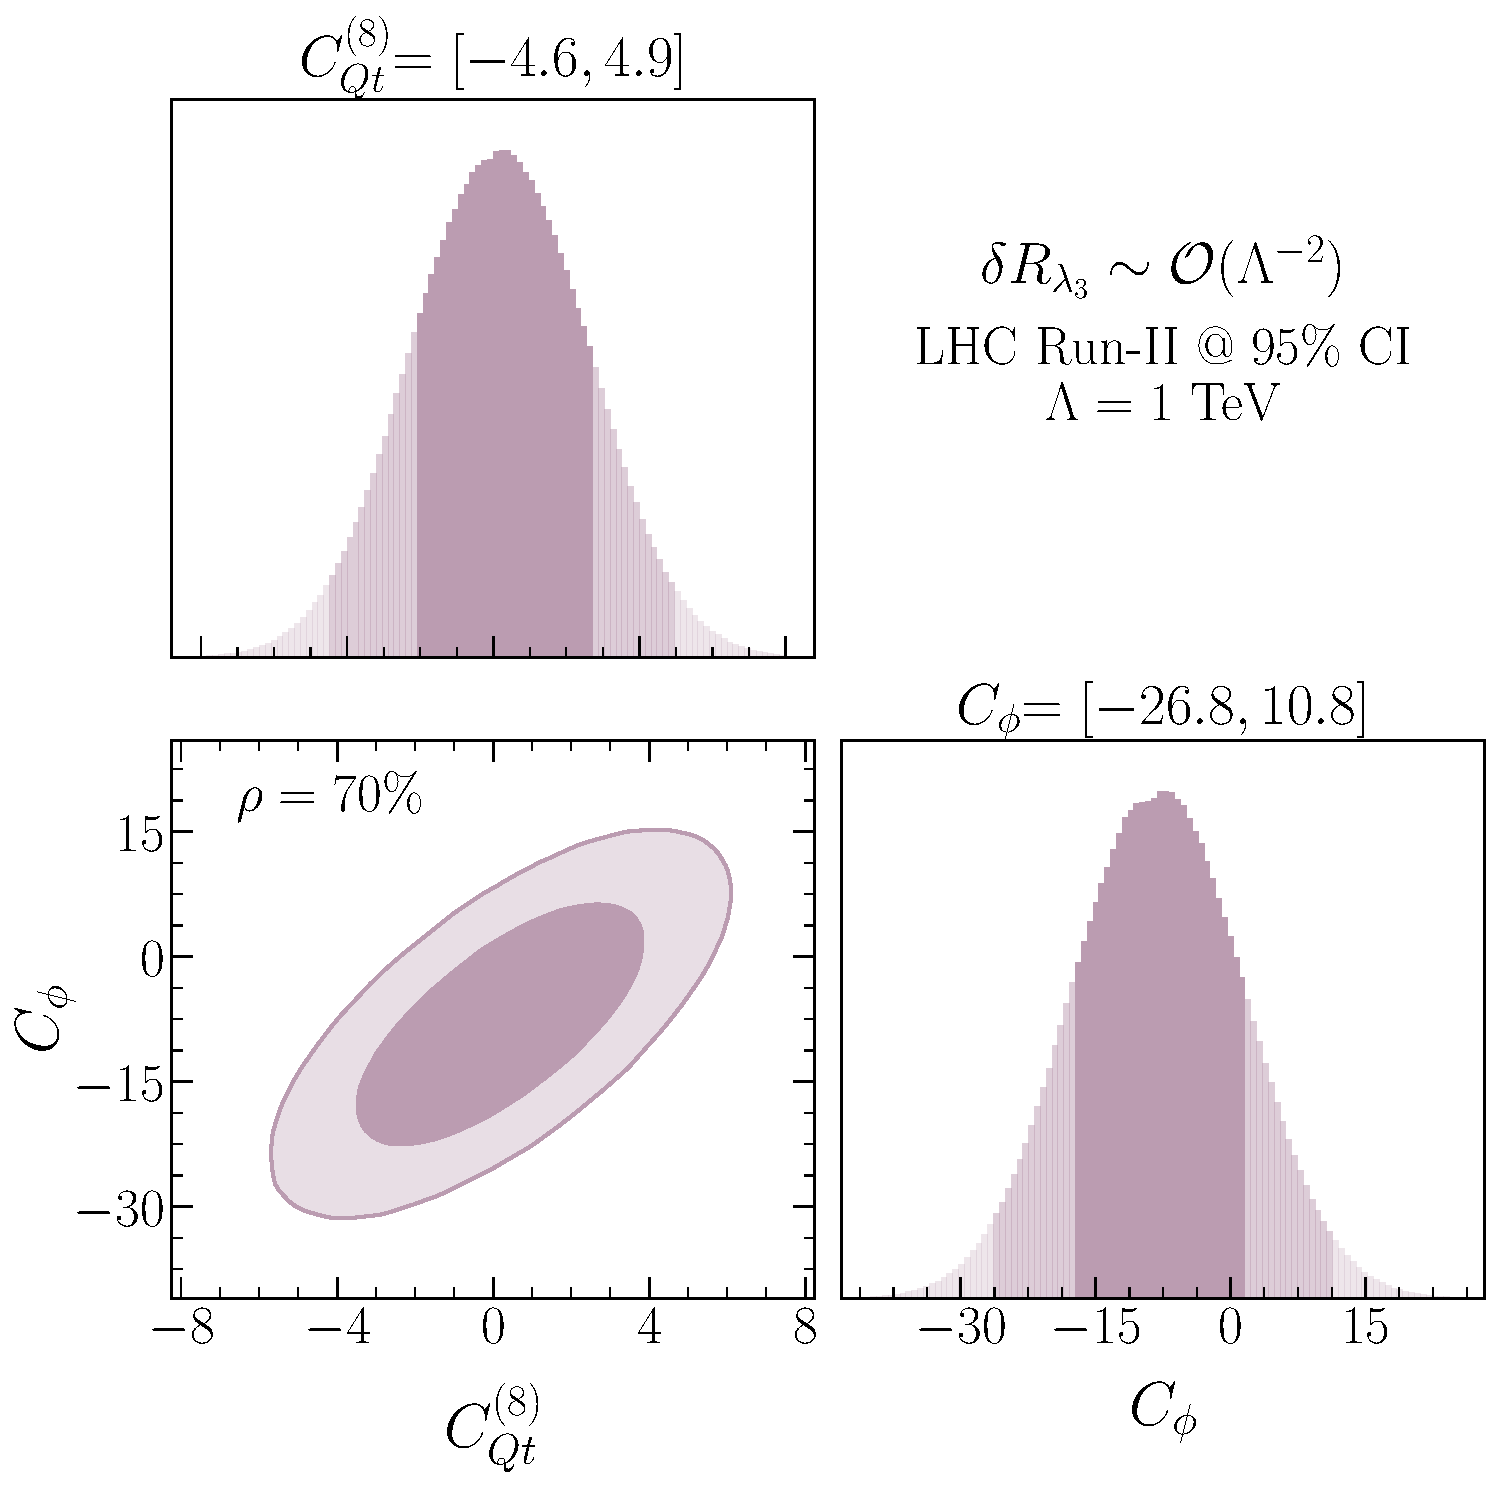
\includegraphics[width=0.45\linewidth]{fig/Cqt8_LHC_RunII_linearl3_rge}
			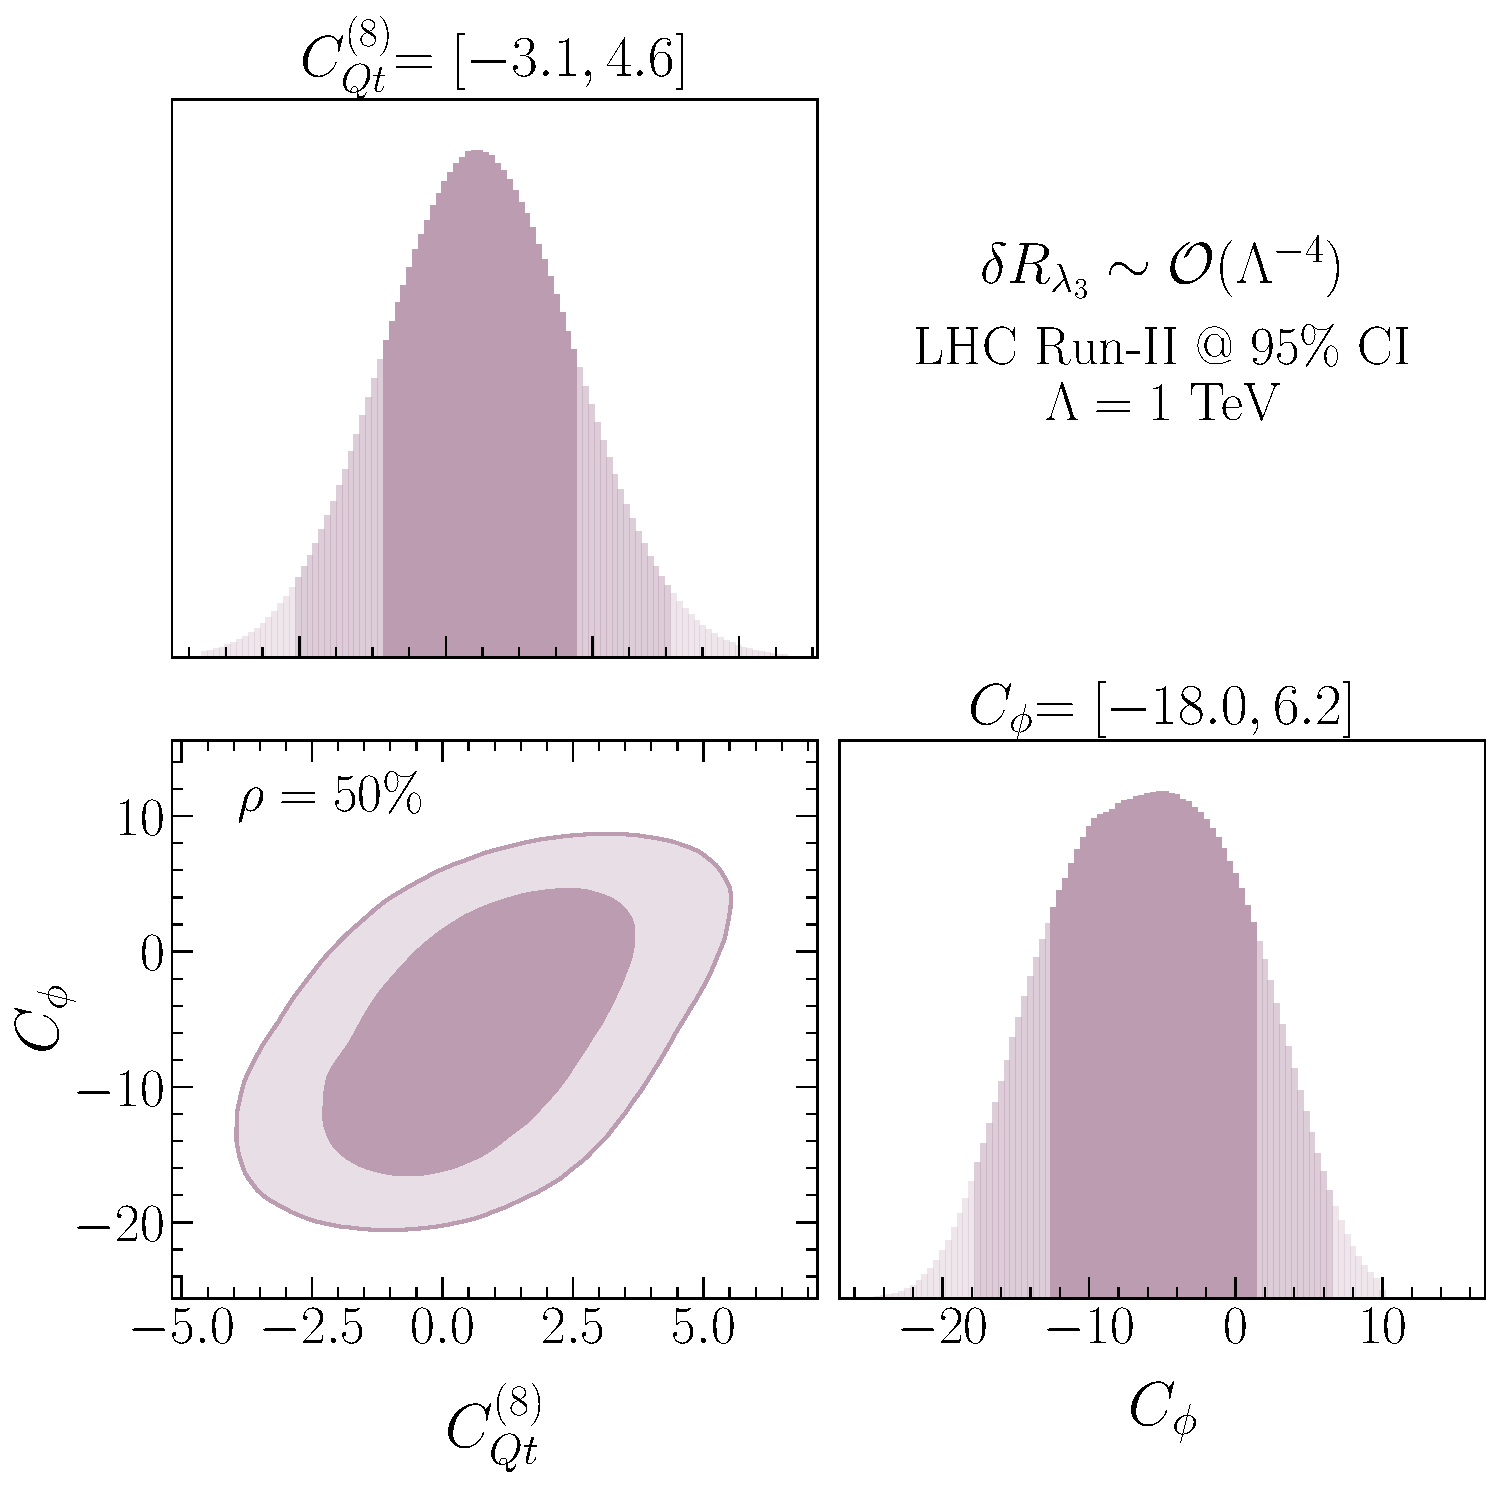
\includegraphics[width=0.45\linewidth]{fig/Cqt8_LHC_RunII_quadl3_rge} 
		\end{center}
		\caption{The posterior distributions of the Run-II data fits for $C_\phi$ with $C_{Qt}^{(1)}$ (up) and $C_\phi$ with $C_{Qt}^{(8)}$ (down). The 68\% and 95\% highest density posterior contours indicated. The limits shown on top of the plots indicate the 95\% CIs. Plots on the left are made for the fully linearised  $\delta R_{\lambda_3}$, while the ones on the right include the quadratic effects. This figure has been published in~\cite{Alasfar:2022zyr}. \label{2param-cqt}   }
	\end{figure}
	
	\begin{figure}[h!]
		\begin{center}
			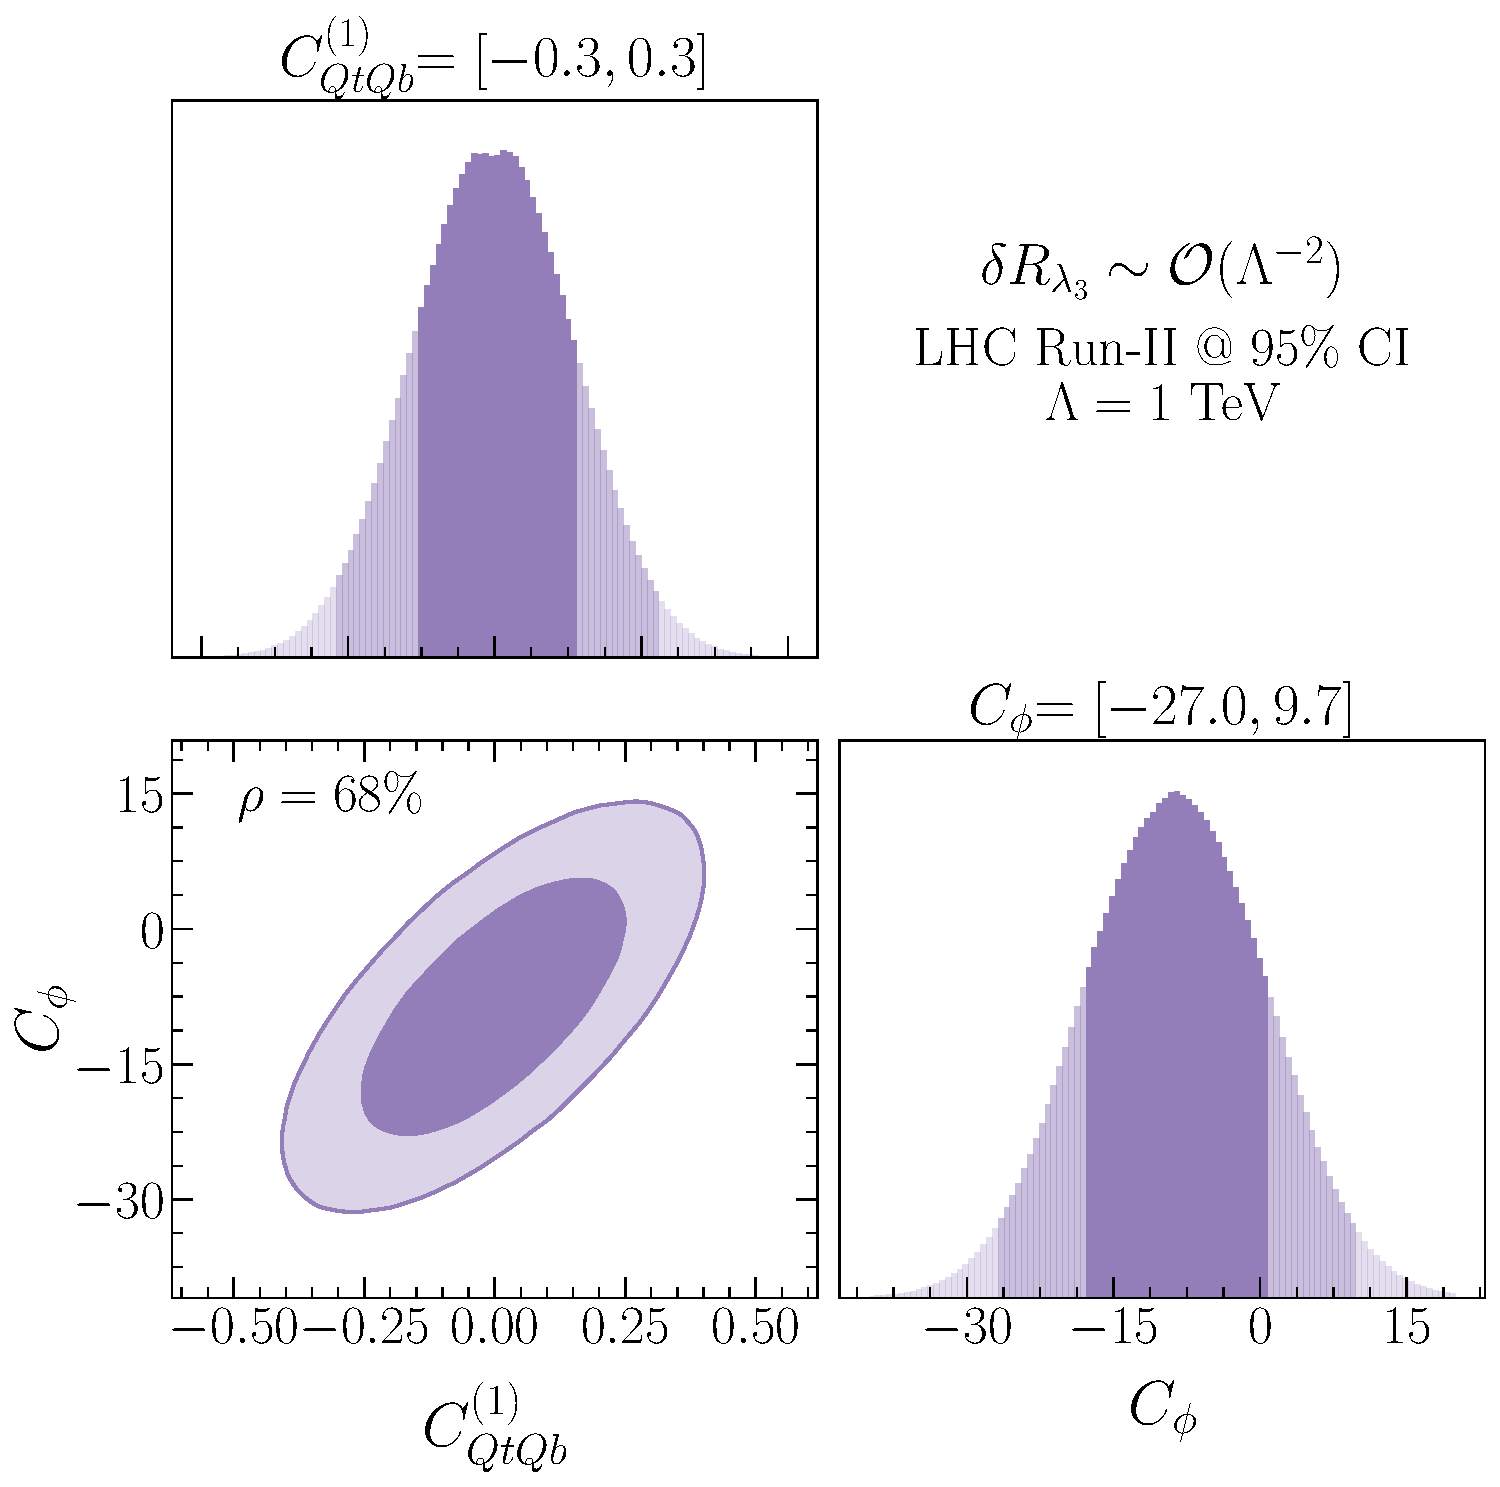
\includegraphics[width=0.45\linewidth]{fig/Cqtqb1_LHC_RunII_linearl3_rge}
			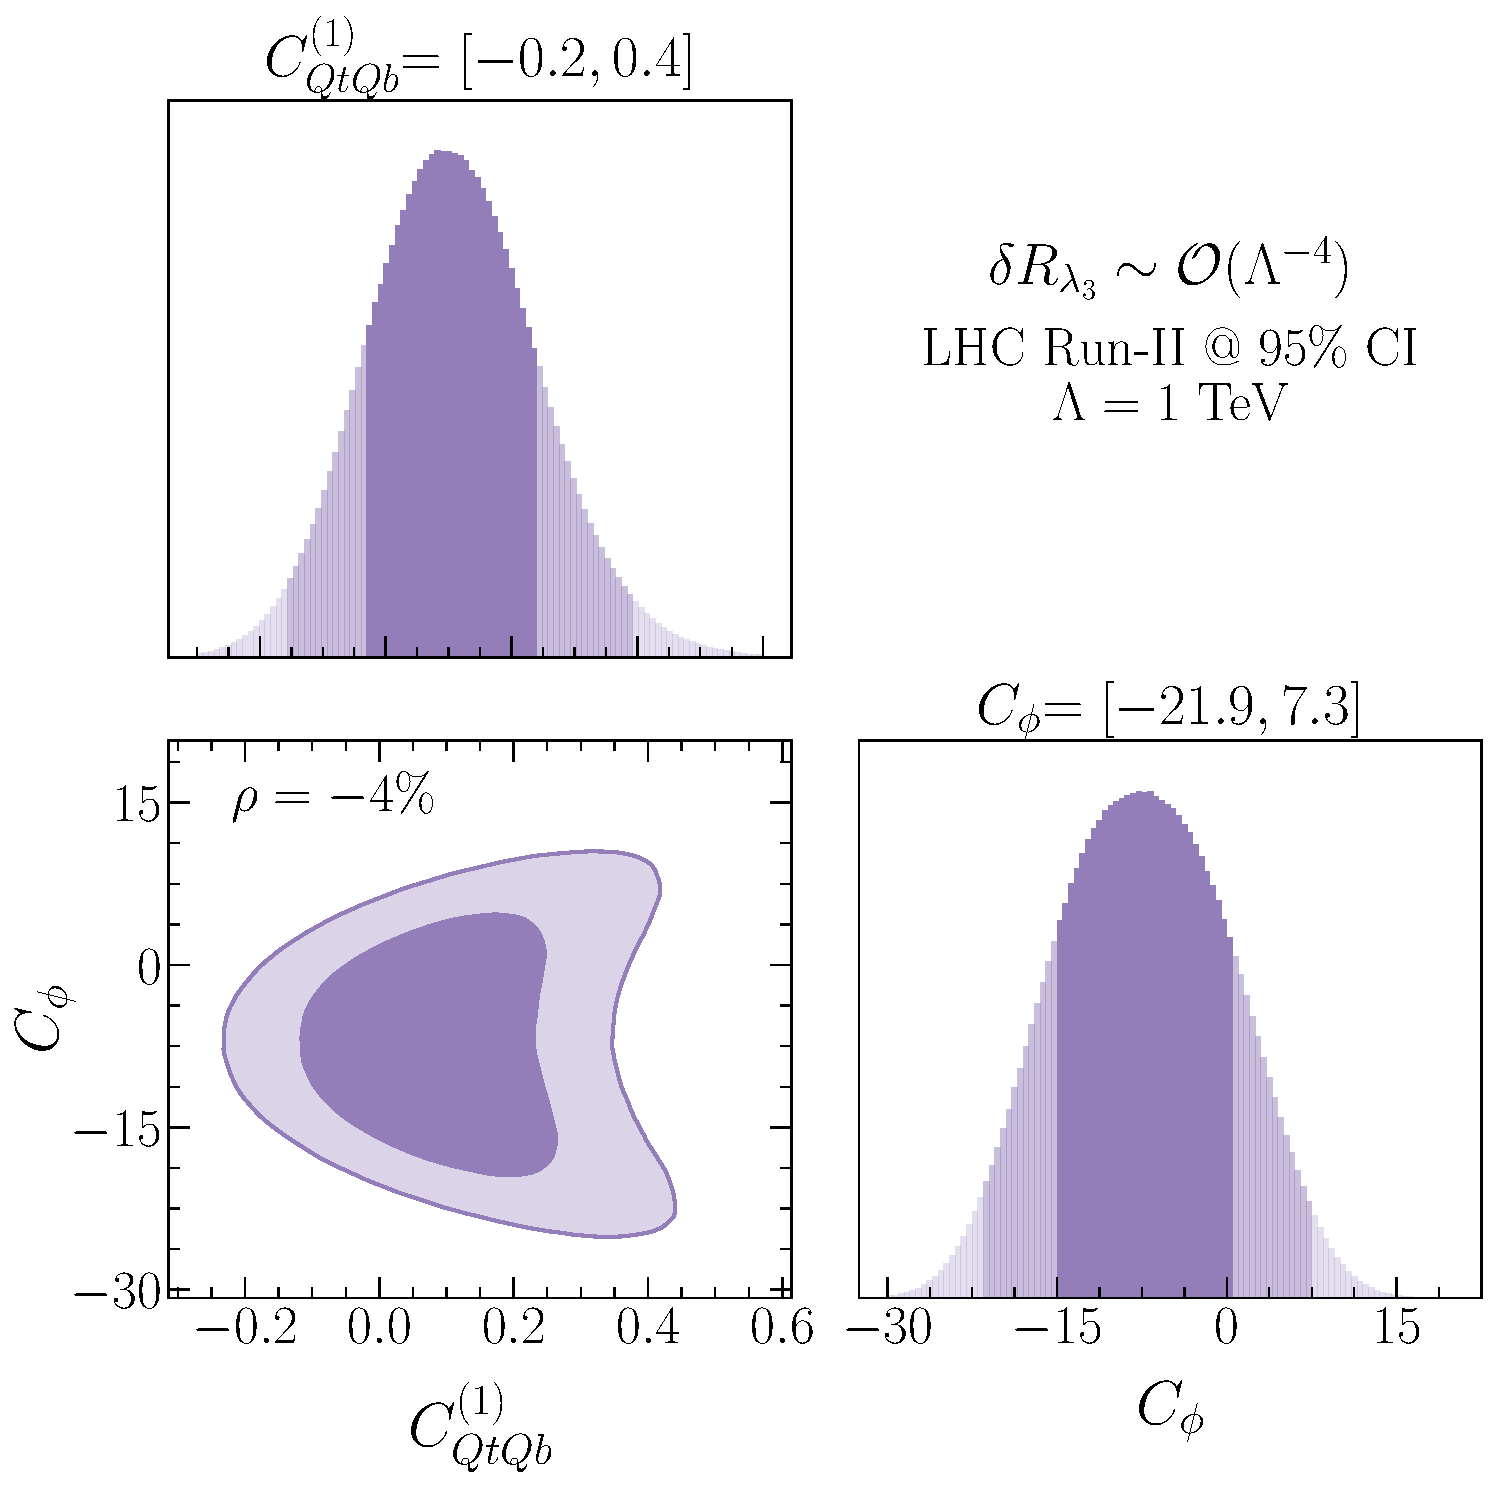
\includegraphics[width=0.45\linewidth]{fig/Cqtqb1_LHC_RunII_quadl3_rge} \\ 
			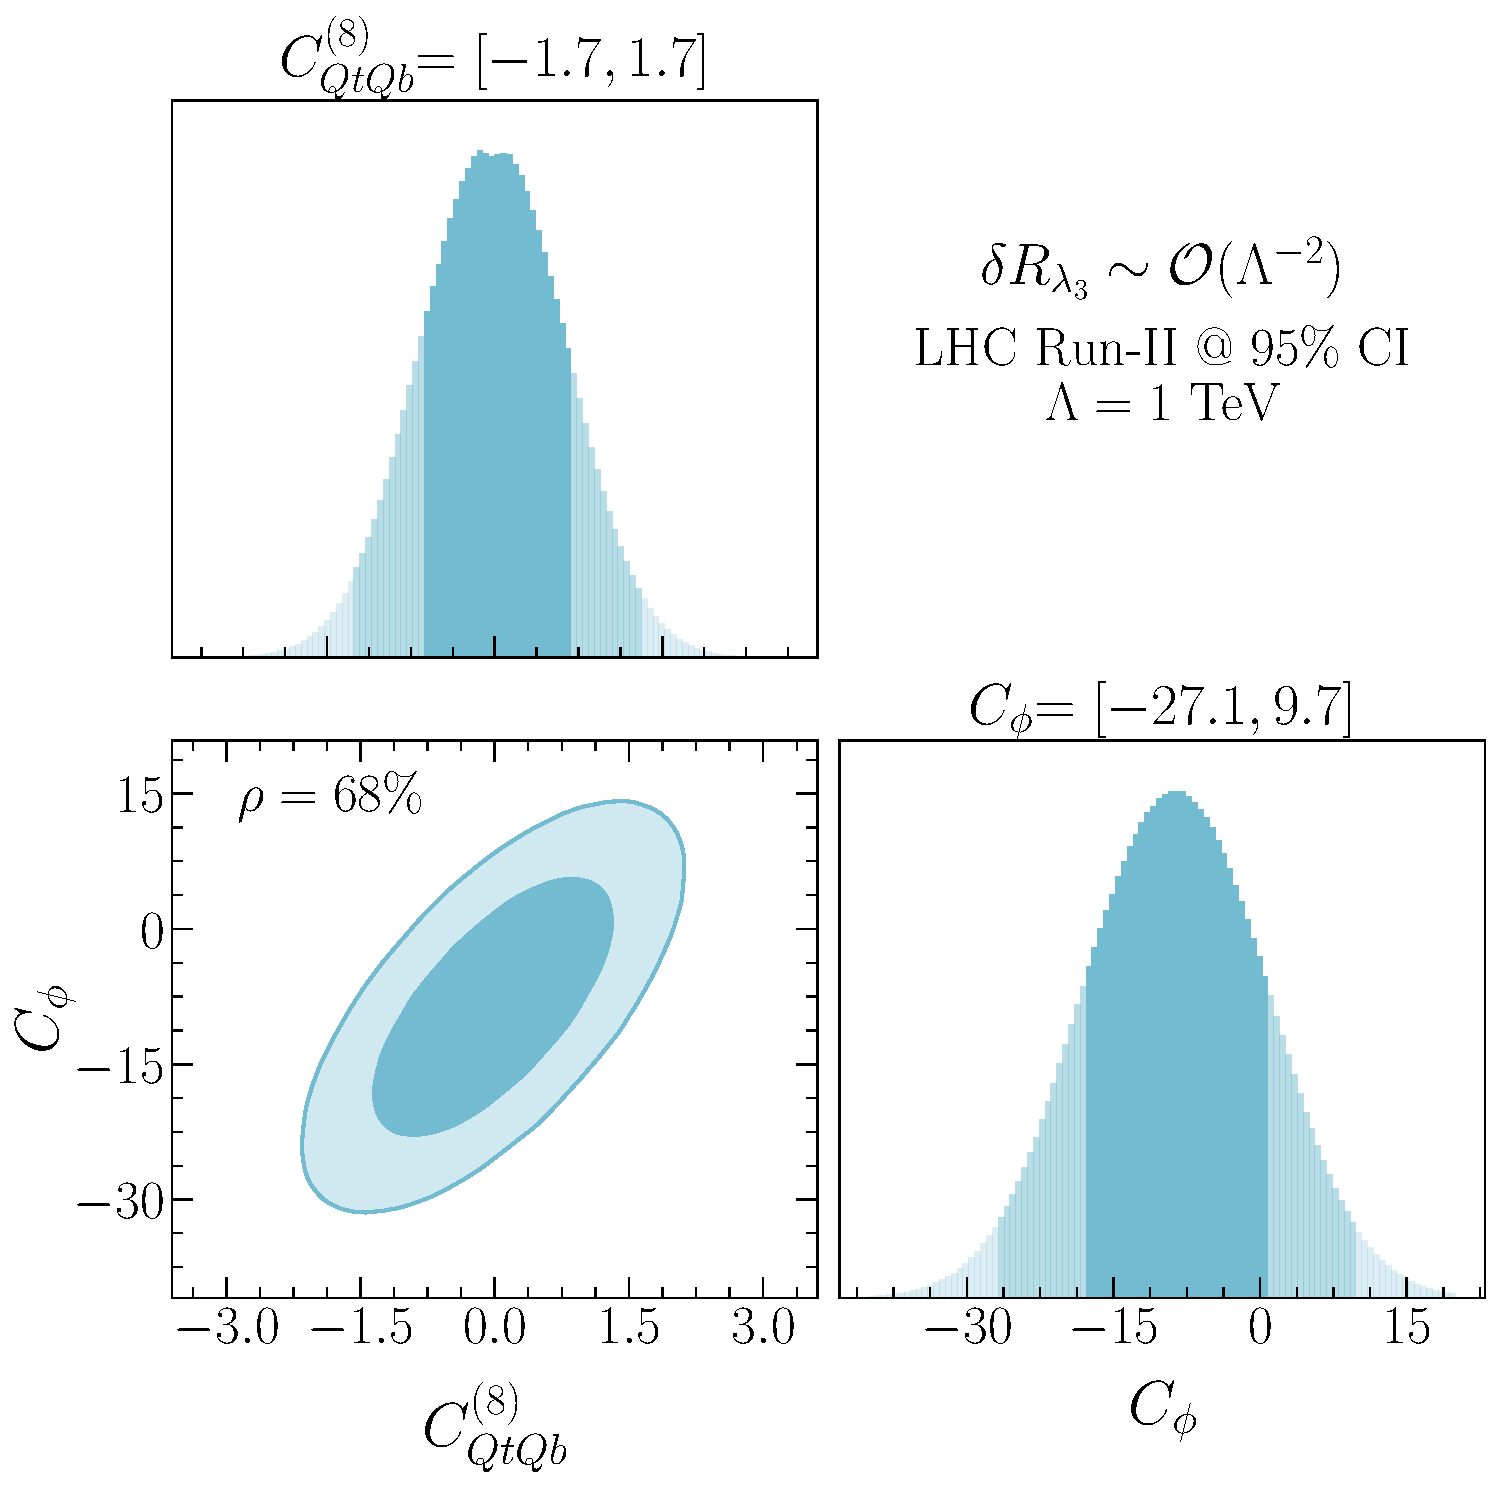
\includegraphics[width=0.45\linewidth]{fig/Cqtqb8_LHC_RunII_linearl3_rge}
			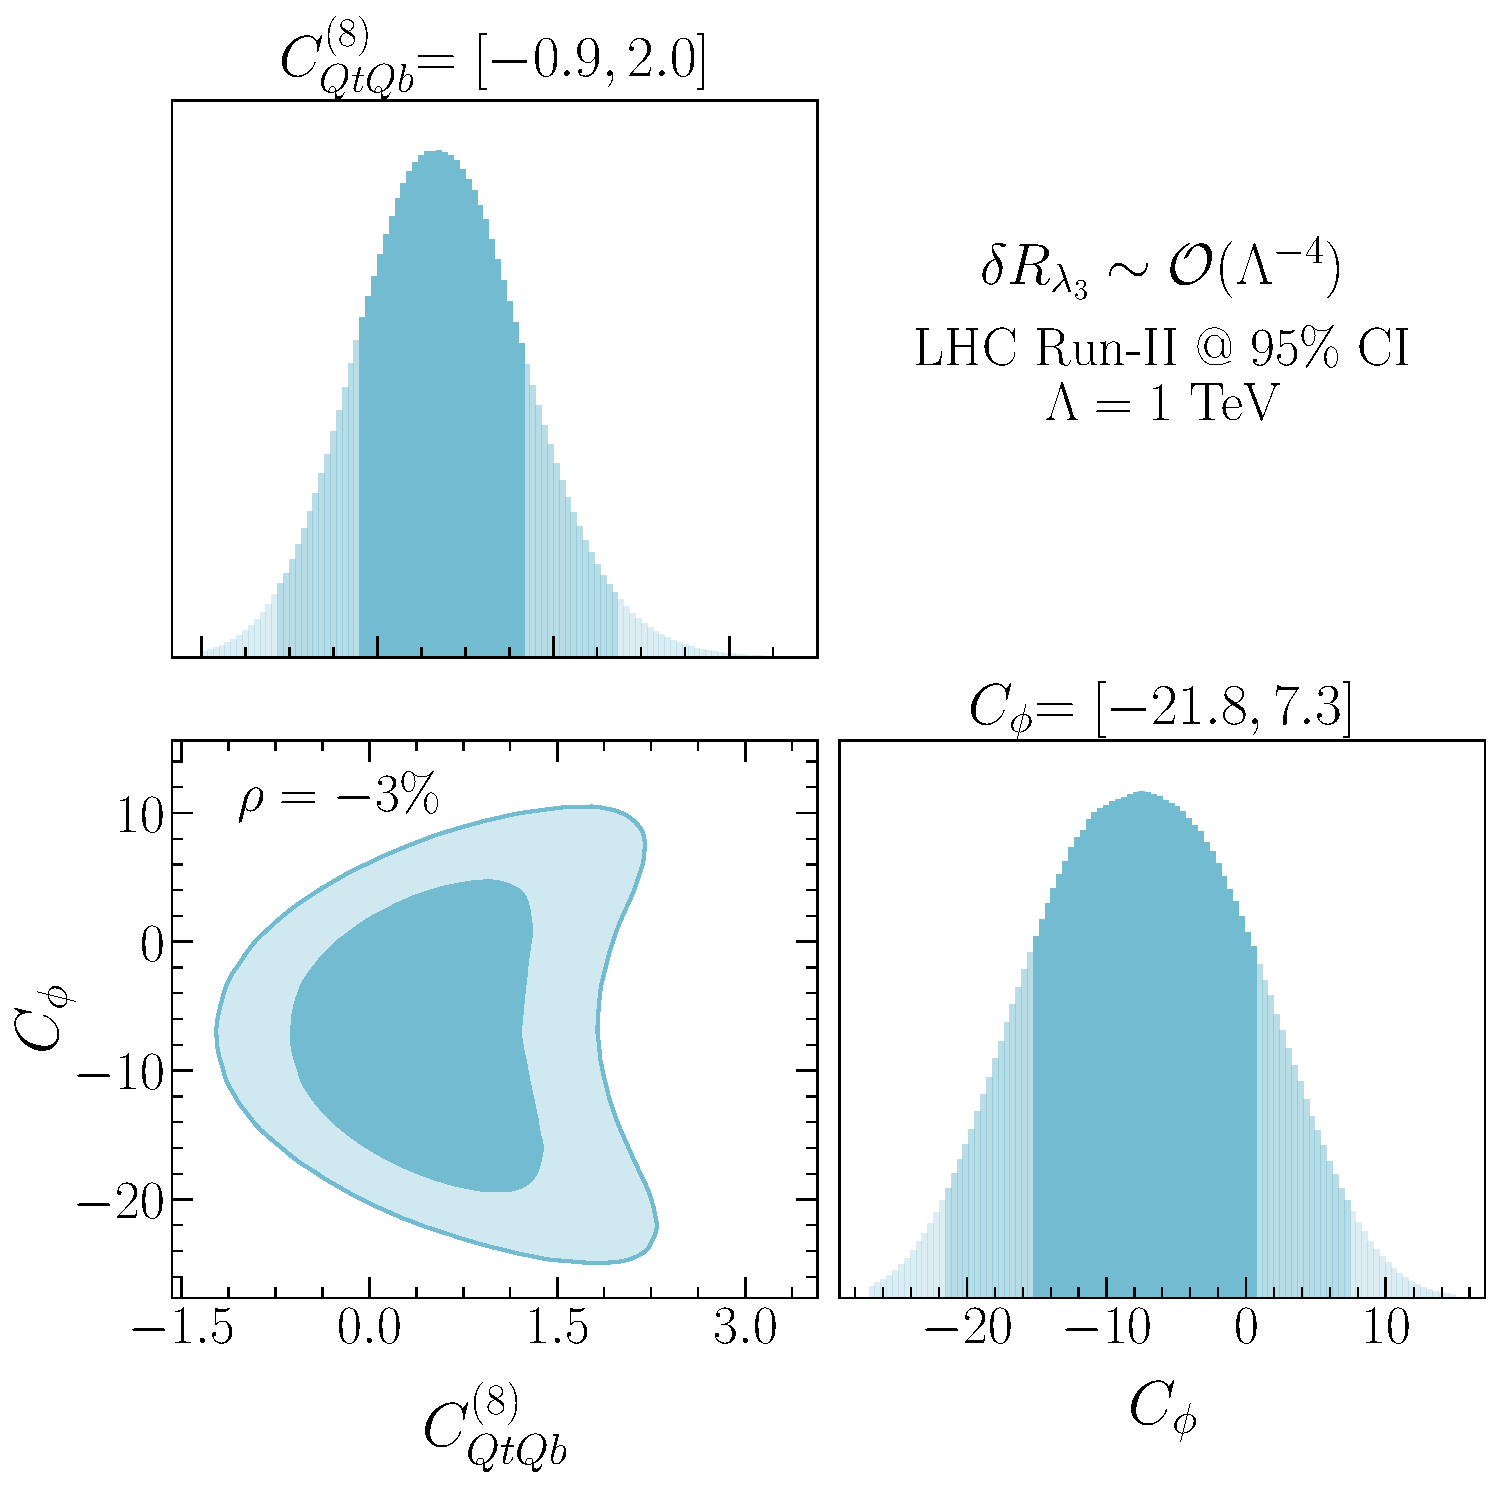
\includegraphics[width=0.45\linewidth]{fig/Cqtqb8_LHC_RunII_quadl3_rge} 
		\end{center}
		\caption{The posterior distributions of the Run-II data fits for $C_\phi$ with $C_{QtQb}^{(1)}$ (up) and $C_\phi$ with $C_{QtQb}^{(8)}$ (down). With the same annotations as in~\autoref{2param-cqt}. This figure has been published in~\cite{Alasfar:2022zyr}. \label{2param-cqtqb}}
	\end{figure}
	We observe that the four-fermion operators are strongly correlated with the Higgs self-coupling modifier~$\mathcal O_\phi$, in the linear fit, with Pearson's correlation of $ \gtrsim 0.7$ and $p$-value $< 10^{-4}$.  In the case of quadratic $\delta R_{\lambda_3}$ fit, we observe diminished Pearson correlation, but in this scenario Pearson's correlation test is not particularly applicable, as we have non-linear relation between the variables.
	%
	\par The two-parameter fit results for the four-fermion Wilson coefficients are summarised in the forest plots in~\autoref{fig:summ4f}, which is obtained by marginalising the posteriors distributions over $C_\phi$. The finite effects were isolated by performing fits with $\delta R^{fin}$ only. The finite effects are small for  $O_{QtQb}^{(1)/(8)}$ but dominant for the four-top operators~$O_{Qt}^{(1)/(8)}$; they are mainly coming from $t\bar t h$.    The effect of EFT truncations of $\delta R_{\lambda_3}$ can also be observed as shifts in the mean values of the Wilson coefficients, but the 95\% CIs themselves are not significantly affected.  In these plots, the fit results from this study are also confronted with the limits obtained from fits to top-quark data \cite{Ethier:2021bye, Ellis:2020unq, Hartland:2019bjb,Brivio:2019ius,DHondt:2018cww, Zhang:2017mls} and EWPO fits from~\cite{Dawson:2022bxd}. When the Wilson coefficient running is taken into account, the 95\% CI  bounds obtained from Higgs data are consistently stronger than the ones from top data.
	\begin{figure}[htpb!]
		\vspace*{-0.5cm}
		\begin{center}
			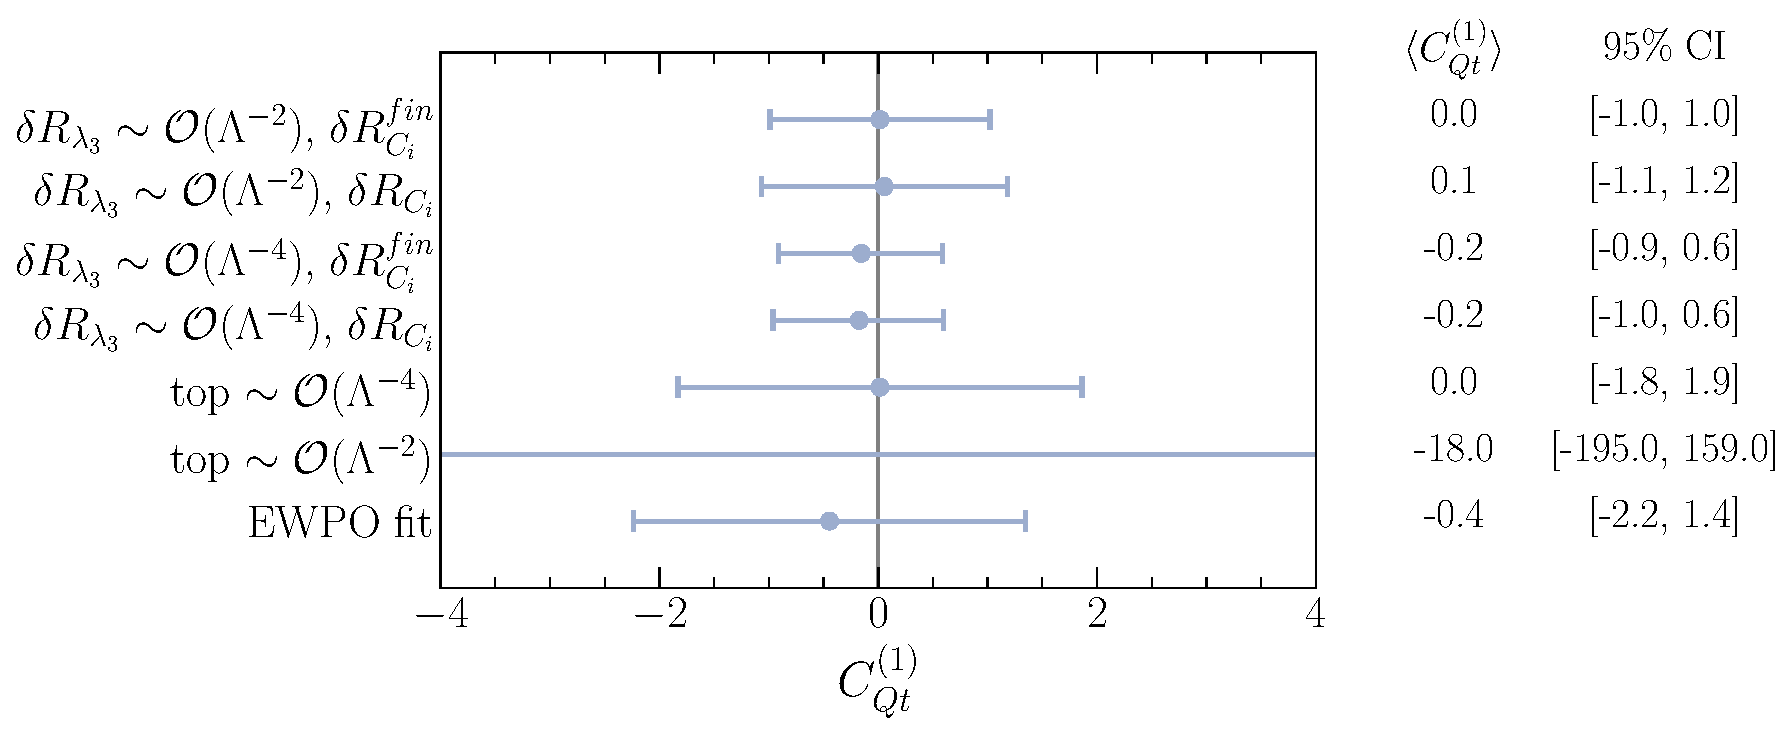
\includegraphics[width=0.75\linewidth]{fig/uebeblick_Cqt1}
			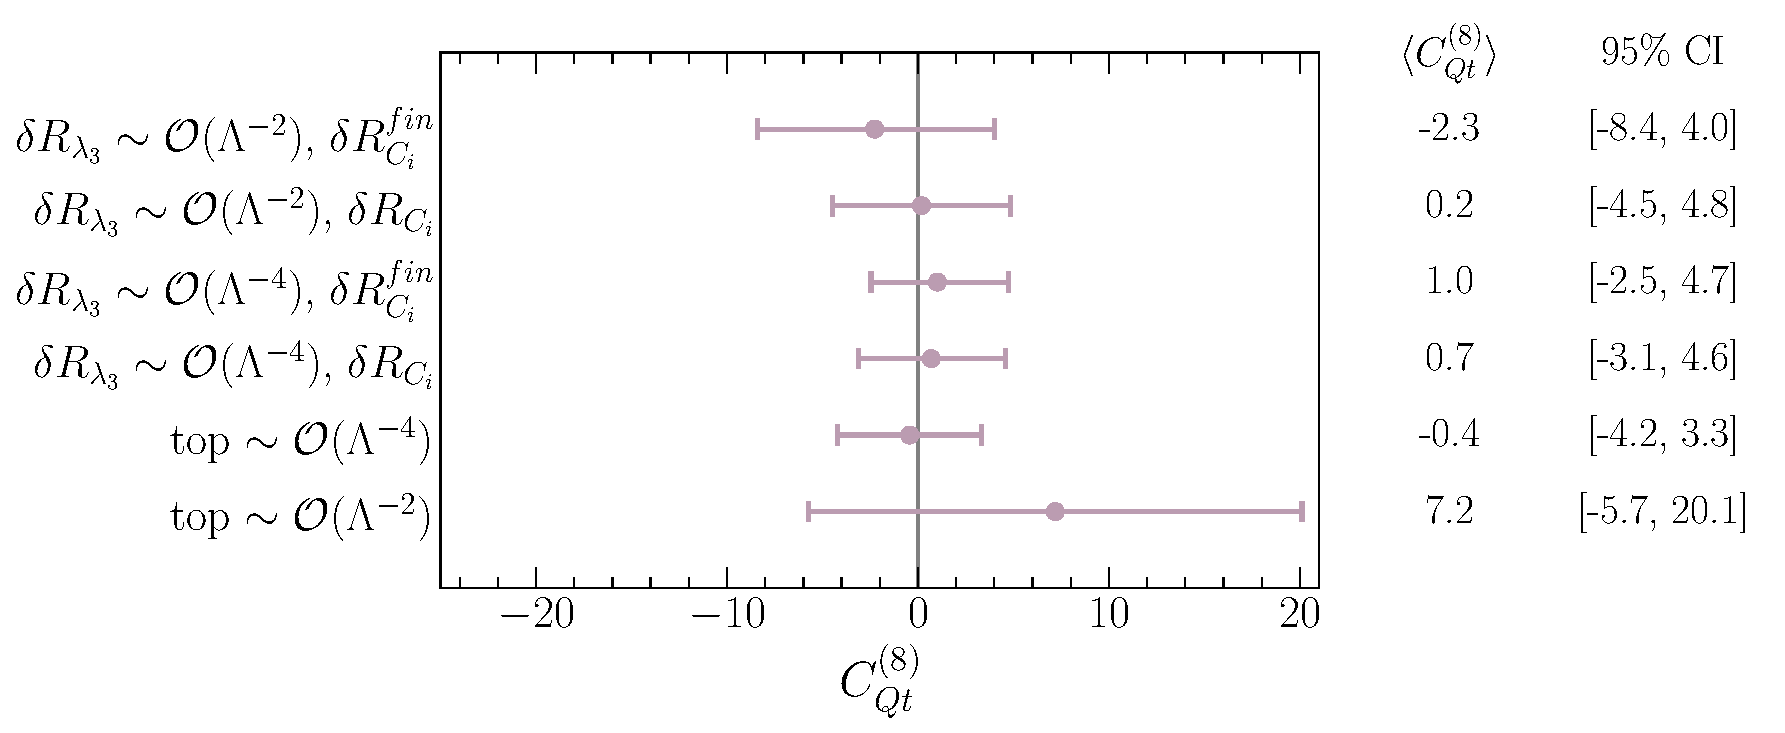
\includegraphics[width=0.75\linewidth]{fig/uebeblick_Cqt8} 
			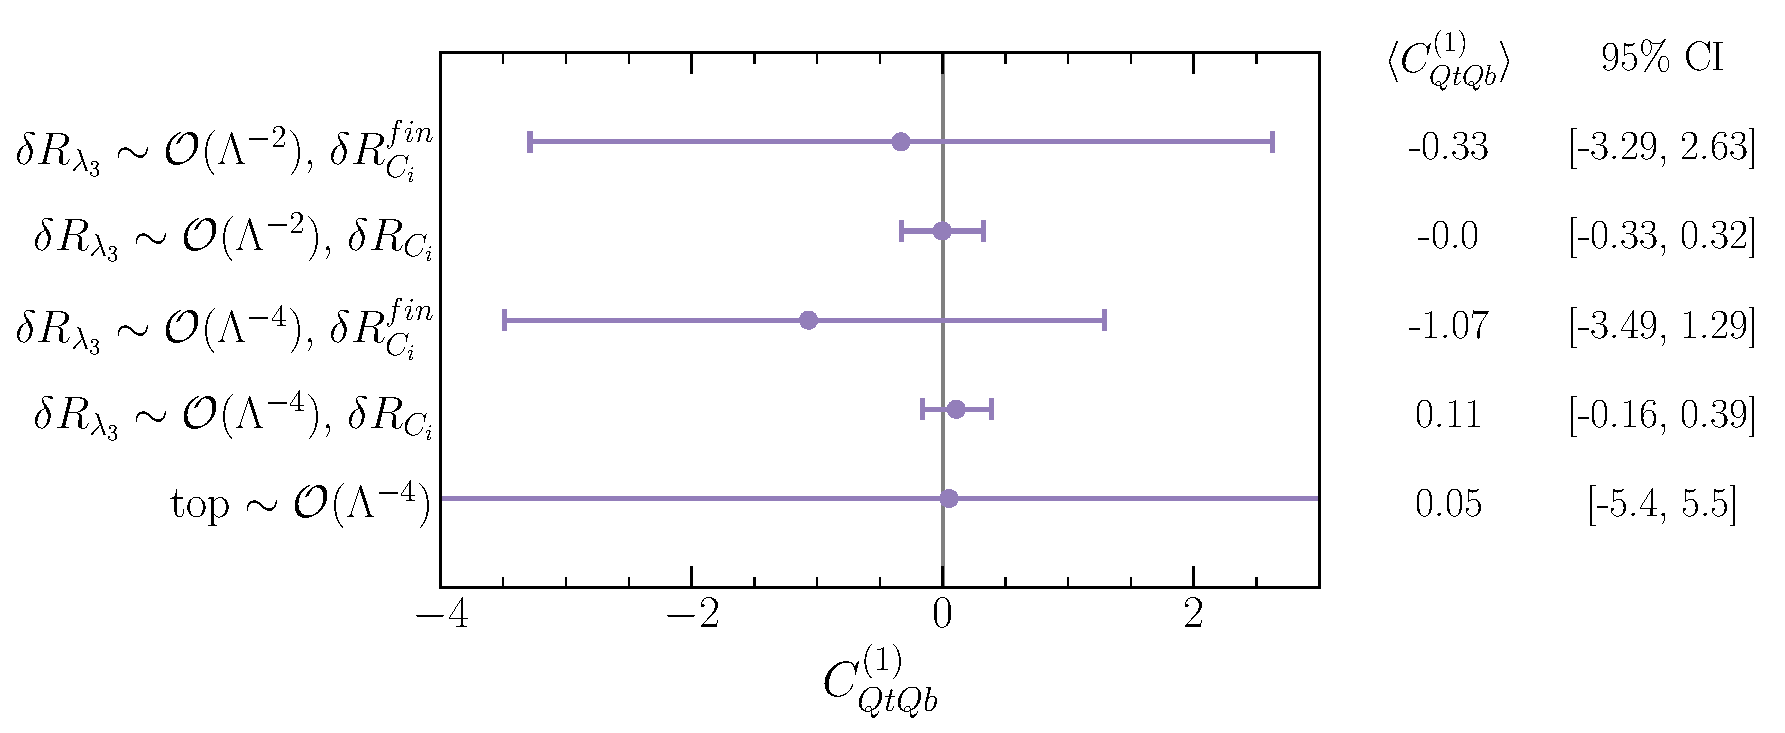
\includegraphics[width=0.75\linewidth]{fig/uebeblick_Cqtqb1}
			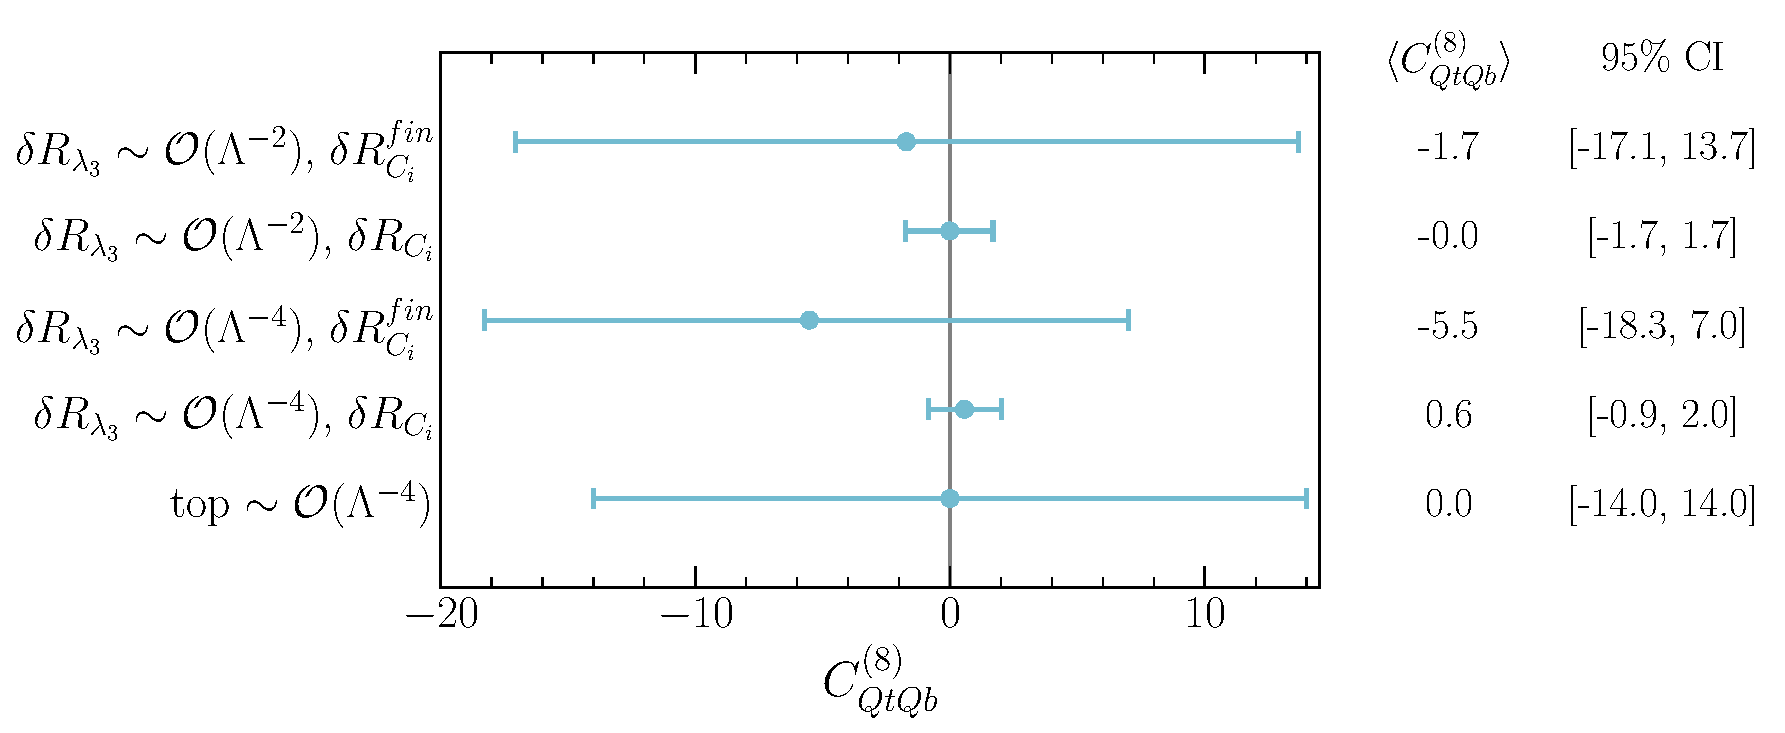
\includegraphics[width=0.75\linewidth]{fig/uebeblick_Cqtqb8}
		\end{center}
		\vspace*{-0.5cm}
		\caption{Forest plots illustrating the means and 95\% CIs constraints on the four-heavy-quark Wilson coefficients $C_i$ from Run-II data. These bounds are obtained from two-parameter fits including the aforementioned coefficients along with $C_\phi$, then marginalising over the latter. The different fits with only the finite part of the NLO correction included vs the full results, as well as the EFT truncation scheme for the trilinear coupling, linear vs quadratic. Fits from top data ~\cite{Ethier:2021bye} for $C_{Qt}^{(1),(8)}$ and~\cite{Hartland:2019bjb} for $C_{QtQb}^{(1),(8)}$ as well as EWPO fits from~\cite{Dawson:2022bxd} were included for comparison. This figure has been published in~\cite{Alasfar:2022zyr}.}
		\label{fig:summ4f}
	\end{figure}
	\par
	 In~\autoref{fig:summcphi},the fit results for~ $C_\phi$ are shown after marginalising over the four-fermion Wilson coefficients in both EFT truncations schemes of $\delta R_{\lambda_3}$, as well as a single parameter fit for~$C_{\phi}$. These fits are compared also to the current 95 \% CL bound on $C_\phi$ extracted from Higgs pair production search using th final state~$b\bar{b} \gamma \gamma$ preformed by ATLAS using Run-II data~\cite{ATLAS:2021jki}, which is translated from $\kappa$ formalism.\\ The mean values and the 95\%CIs change depending on the four-fermion Wilson coefficient that was paired with $C_\phi$ in the two-parameter fits. As expected, the single parameter fits for $C_\phi$ yield stronger bound on $C_\phi$ than the two-parameter fits, thus the inclusion of the four-fermion operators in single Higgs data dilutes $C_\phi$ bounds.  Additionally, the truncation order of  $\delta R_{\lambda_3}$ appears to have a marked effect on the length of the CIs, with quadratic fits giving more stringent constraints on $C_\phi$. Instead, for Higgs pair production  is makes only a negligible effect  if linear or up to quadratic terms in the EFT expansion are kept  for the $C_\phi>0$ bound, while the bound weakens at linear order in $1/\Lambda^2$ for $C_\phi<0$~\cite{IML}. For instance, the quadratic single parameter fit for $C_\phi$ is comparable to the direct bound from Higgs pair production. However, this changes dramatically, when one includes the four-fermion operators in a combined fit, and the single-Higgs data constraints on $C_\phi$ become less significant compared to the direct $hh$ bounds. \\
	It should be noted that the strongest bond on the Higgs self-coupling currently comes from the perturbative unitarity bound of ref.~\cite{DiLuzio:2017tfn}.
	\begin{figure}[htpb!]
		\begin{center}
			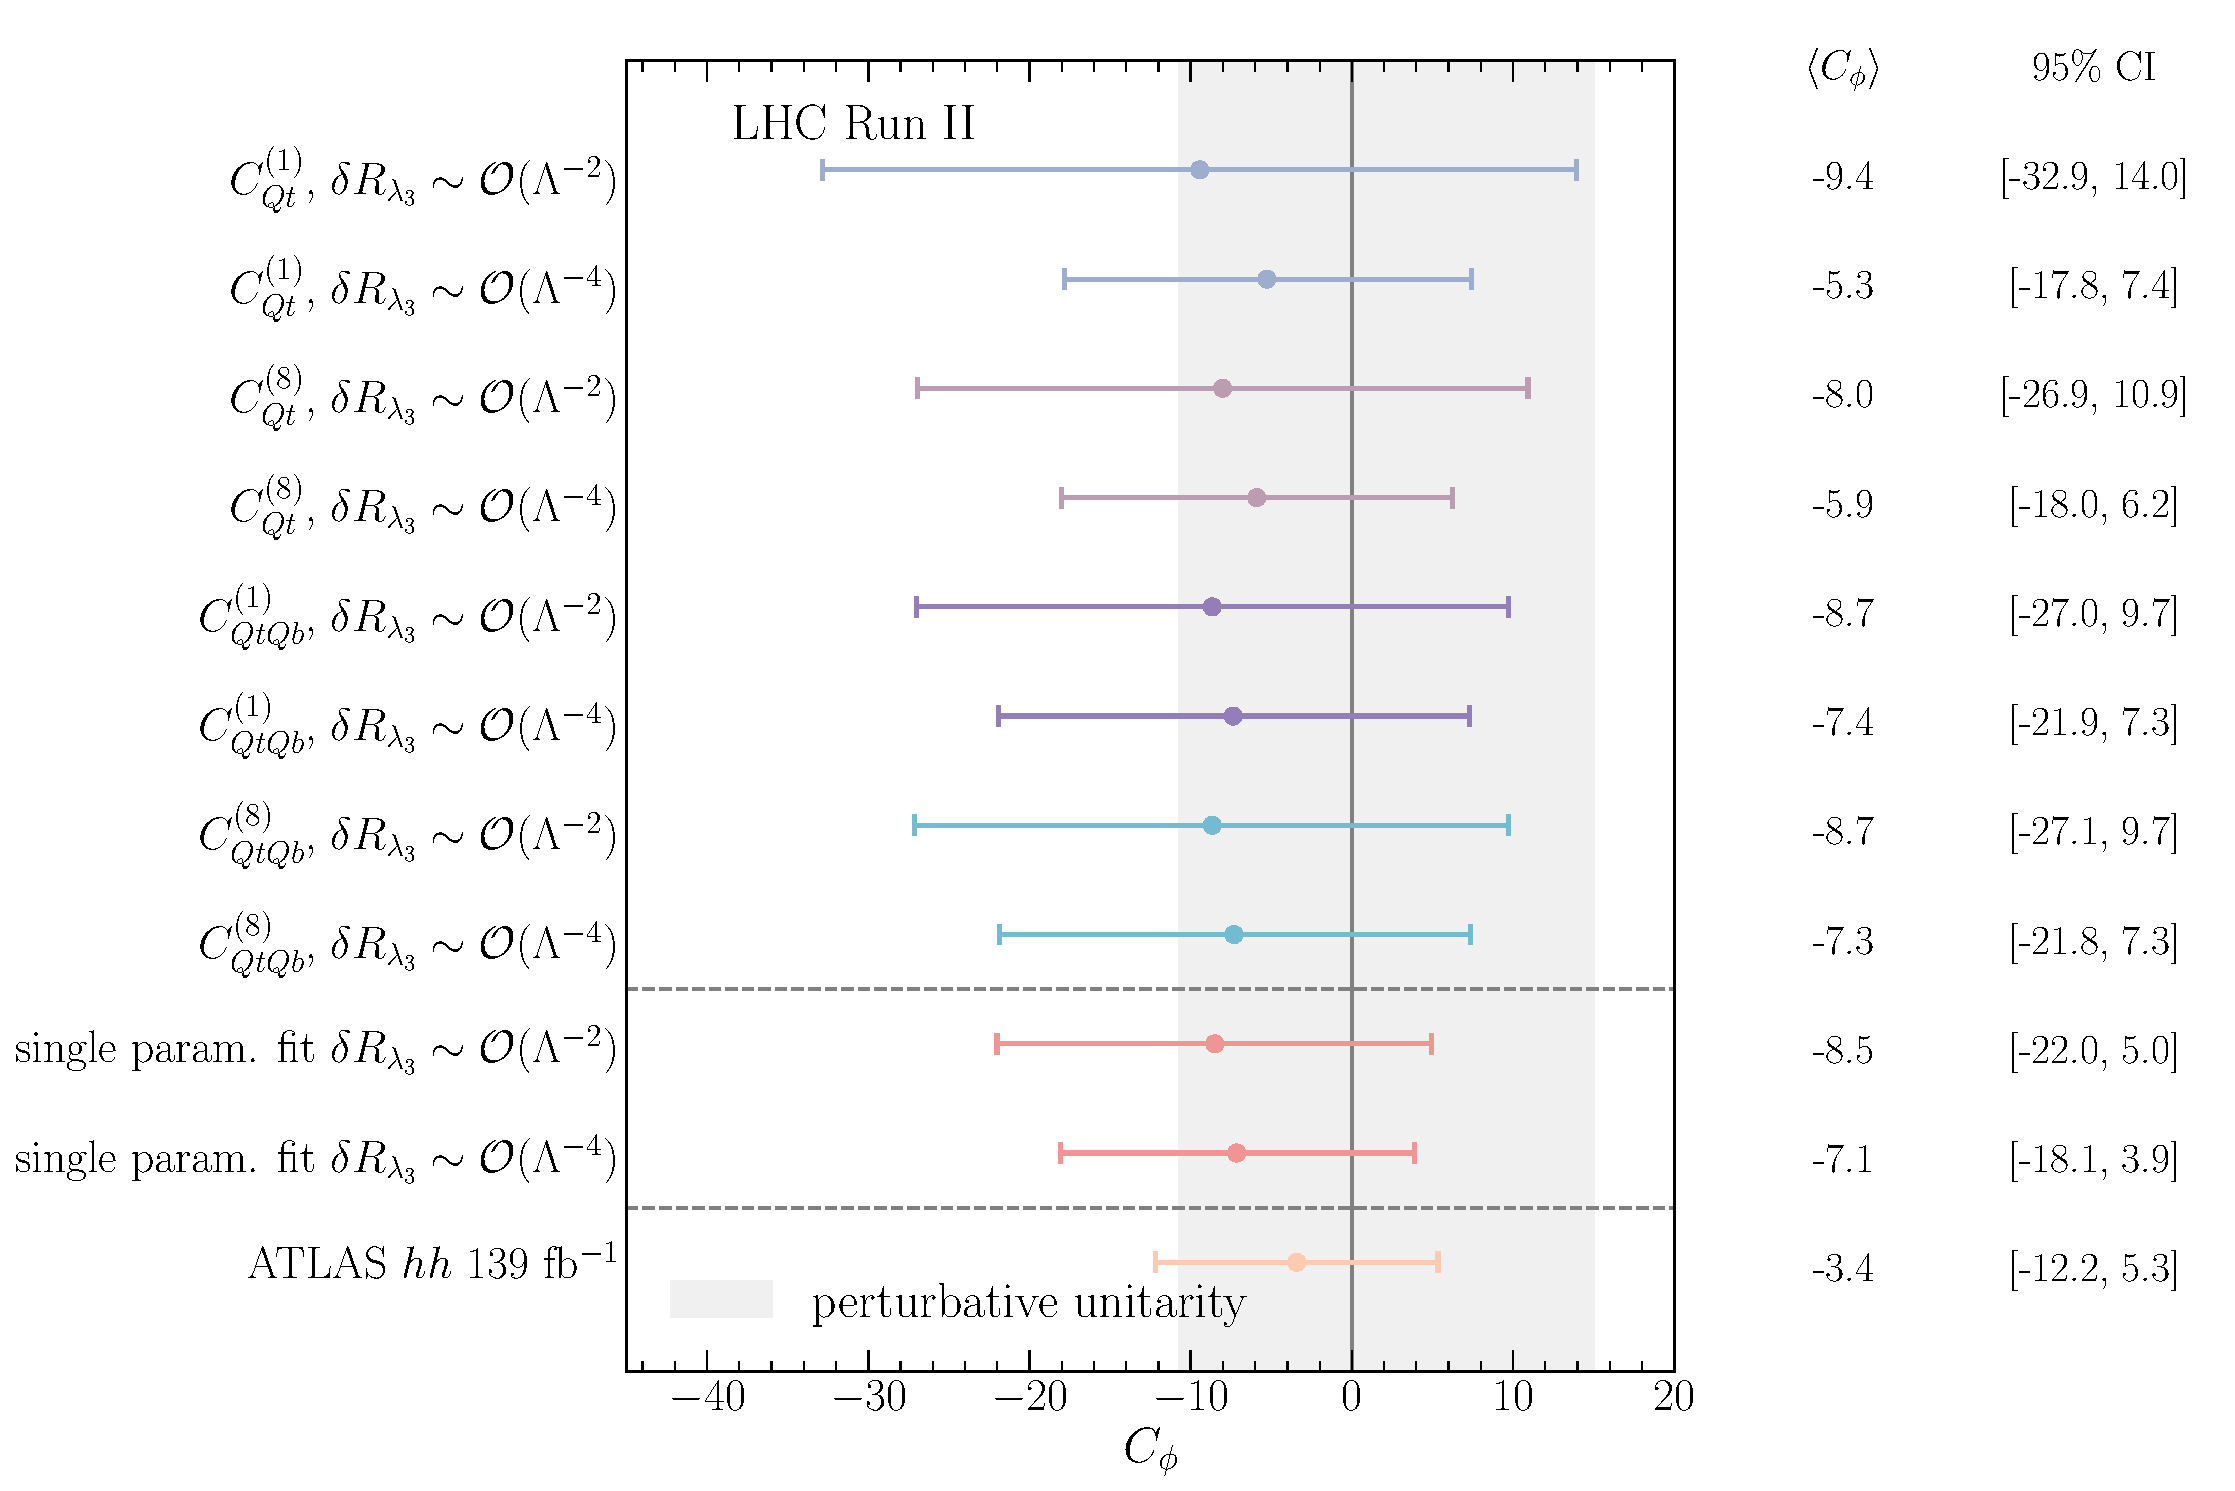
\includegraphics[width=\linewidth]{fig/uebeblick_forest_cphi_LHC_RunII}
		\end{center}
		\caption{A forest plot illustrating the means and 95\% CIs bounds for $C_\phi$ from the two-parameter fit, with the four-fermion operators marginalised. The fits results for $C_\phi$ from full Run-II Higgs data keeping terms up to $\mathcal{O}(1/\Lambda^2)$ or $\mathcal{O}(1/\Lambda^4)$ in $\delta R_{\lambda_3}$ are shown.  For comparison, also the 95\% CI and means for the single parameter fit for $C_\phi$ with the same single Higgs data is shown as well as the bounds on $C_{\phi}$ from the $139$ fb$^{-1}$ search for Higgs pair production~\cite{ATLAS:2021jki}. The horizontal grey band highlights the perturbative unitarity bound~\cite{DiLuzio:2017tfn}. This figure has been published in~\cite{Alasfar:2022zyr}.\label{fig:summcphi}  }
	\end{figure}
	%%%%%%%%%%%%%%%%%%%
	\par 
	One of the important aspects of multivariate studies is the correlation between the variables. Apart from the two-parameter fits discussed above, four-parameter fits are also considered. These fits include $C_\phi$ plus the three directions in the four heavy-quark operator parameter spaces that the Higgs rates are
	mostly sensitive too, i.e. neglecting $C_{QQ}^{(1),(3) }$ and $C_{tt}$, and trading $C_{QtQb}^{(1)}$ and $C_{QtQb}^{(8)}$ by $C_{QtQb}^{+}$.
	%%%%%%%%%%
	\begin{figure}[h!]
		\begin{center}
			%	\vspace{-1.5cm}
			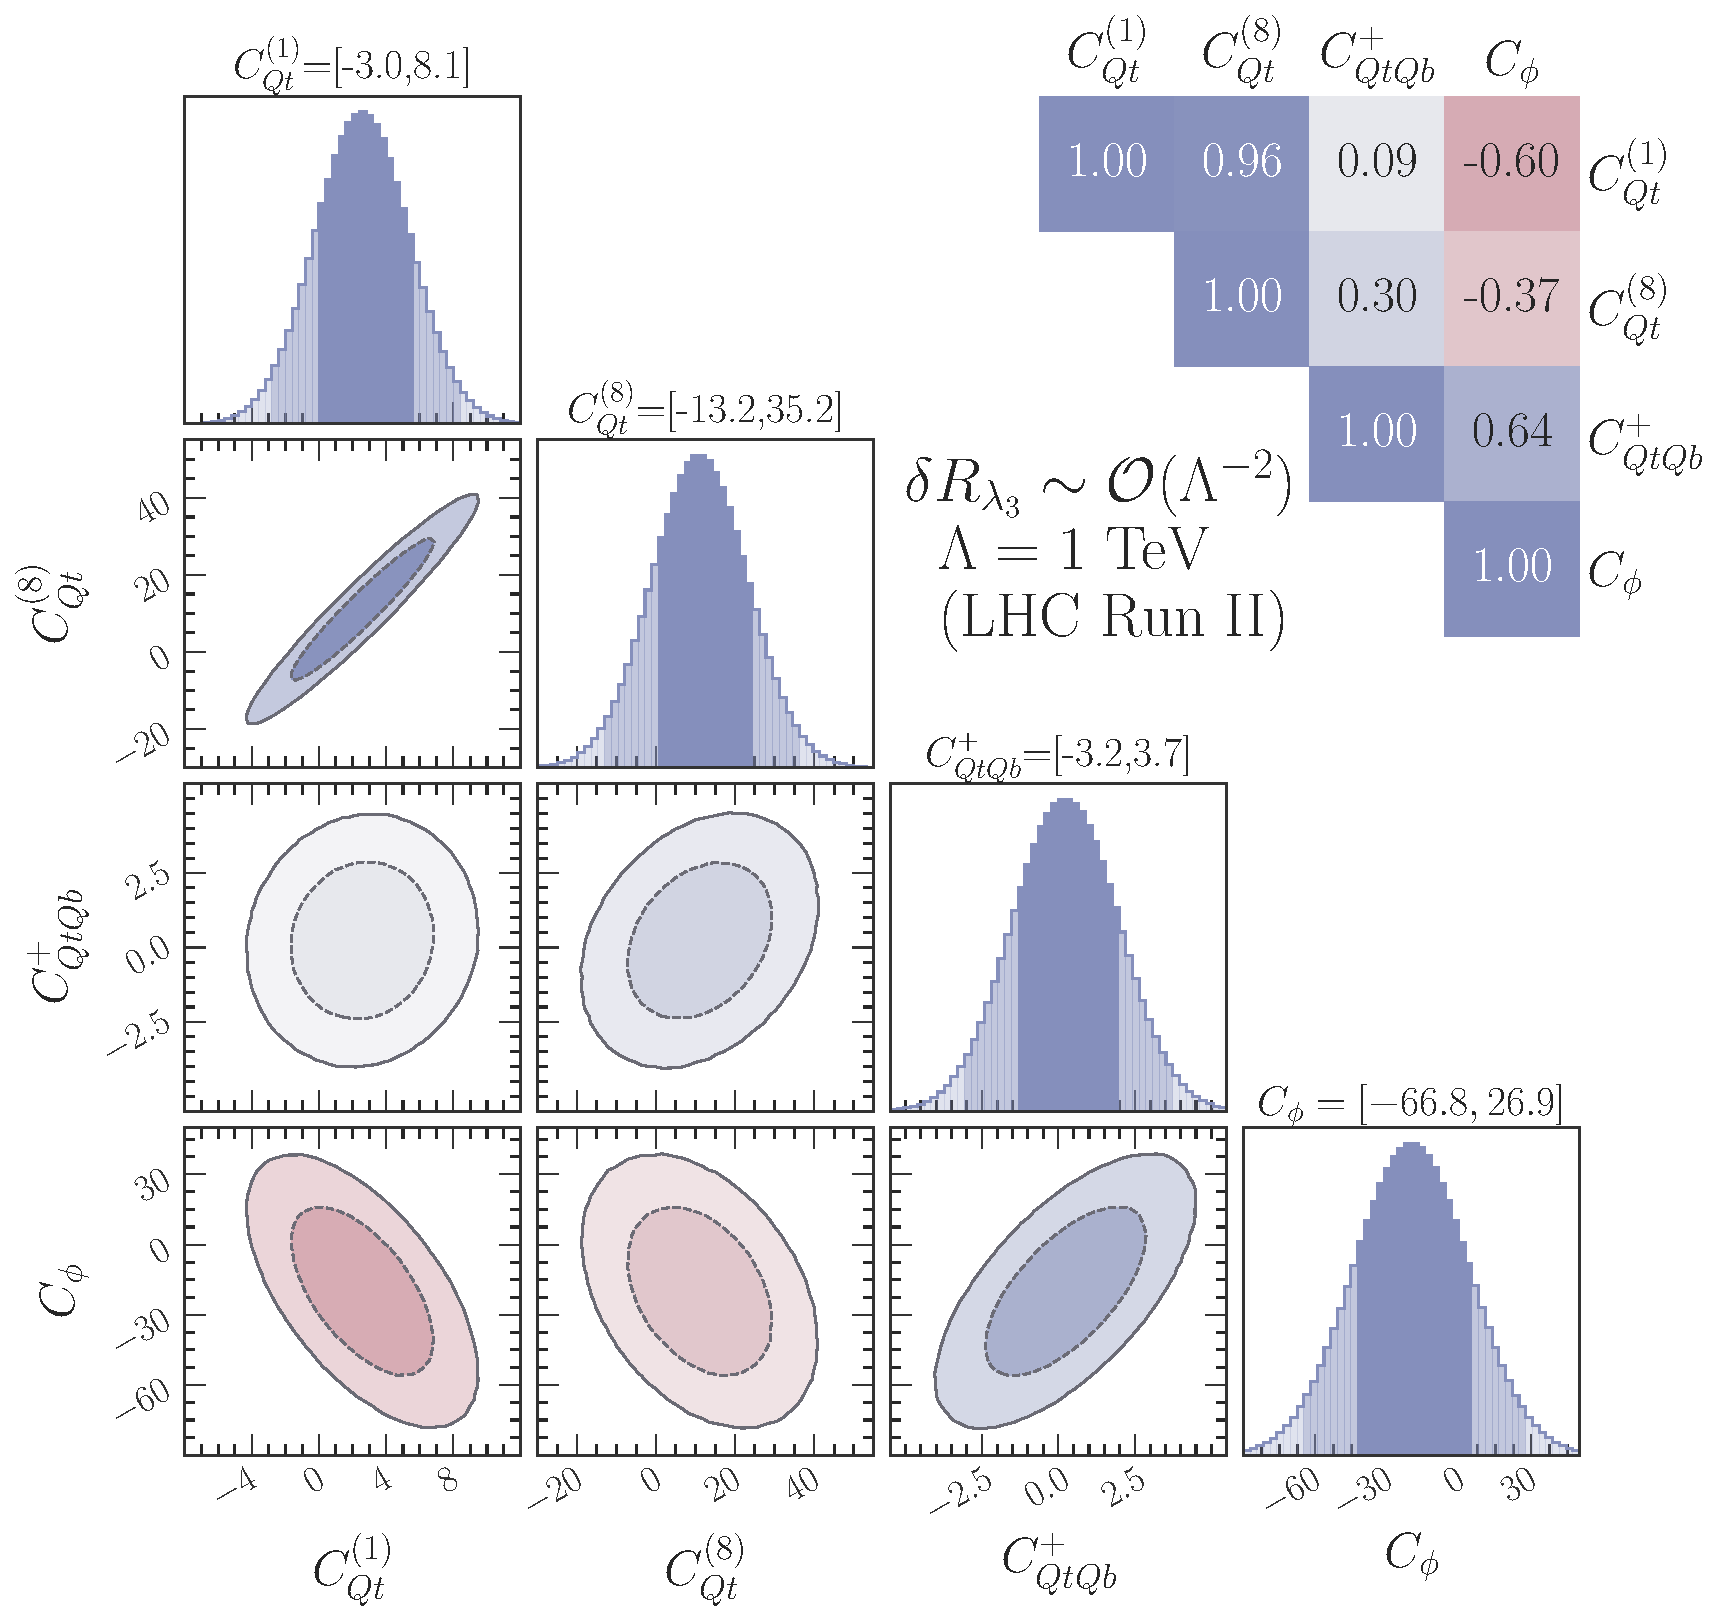
\includegraphics[width=.6\linewidth]{fig/4param_fit_LHC_RunII_l3L_rge}\\
			%
			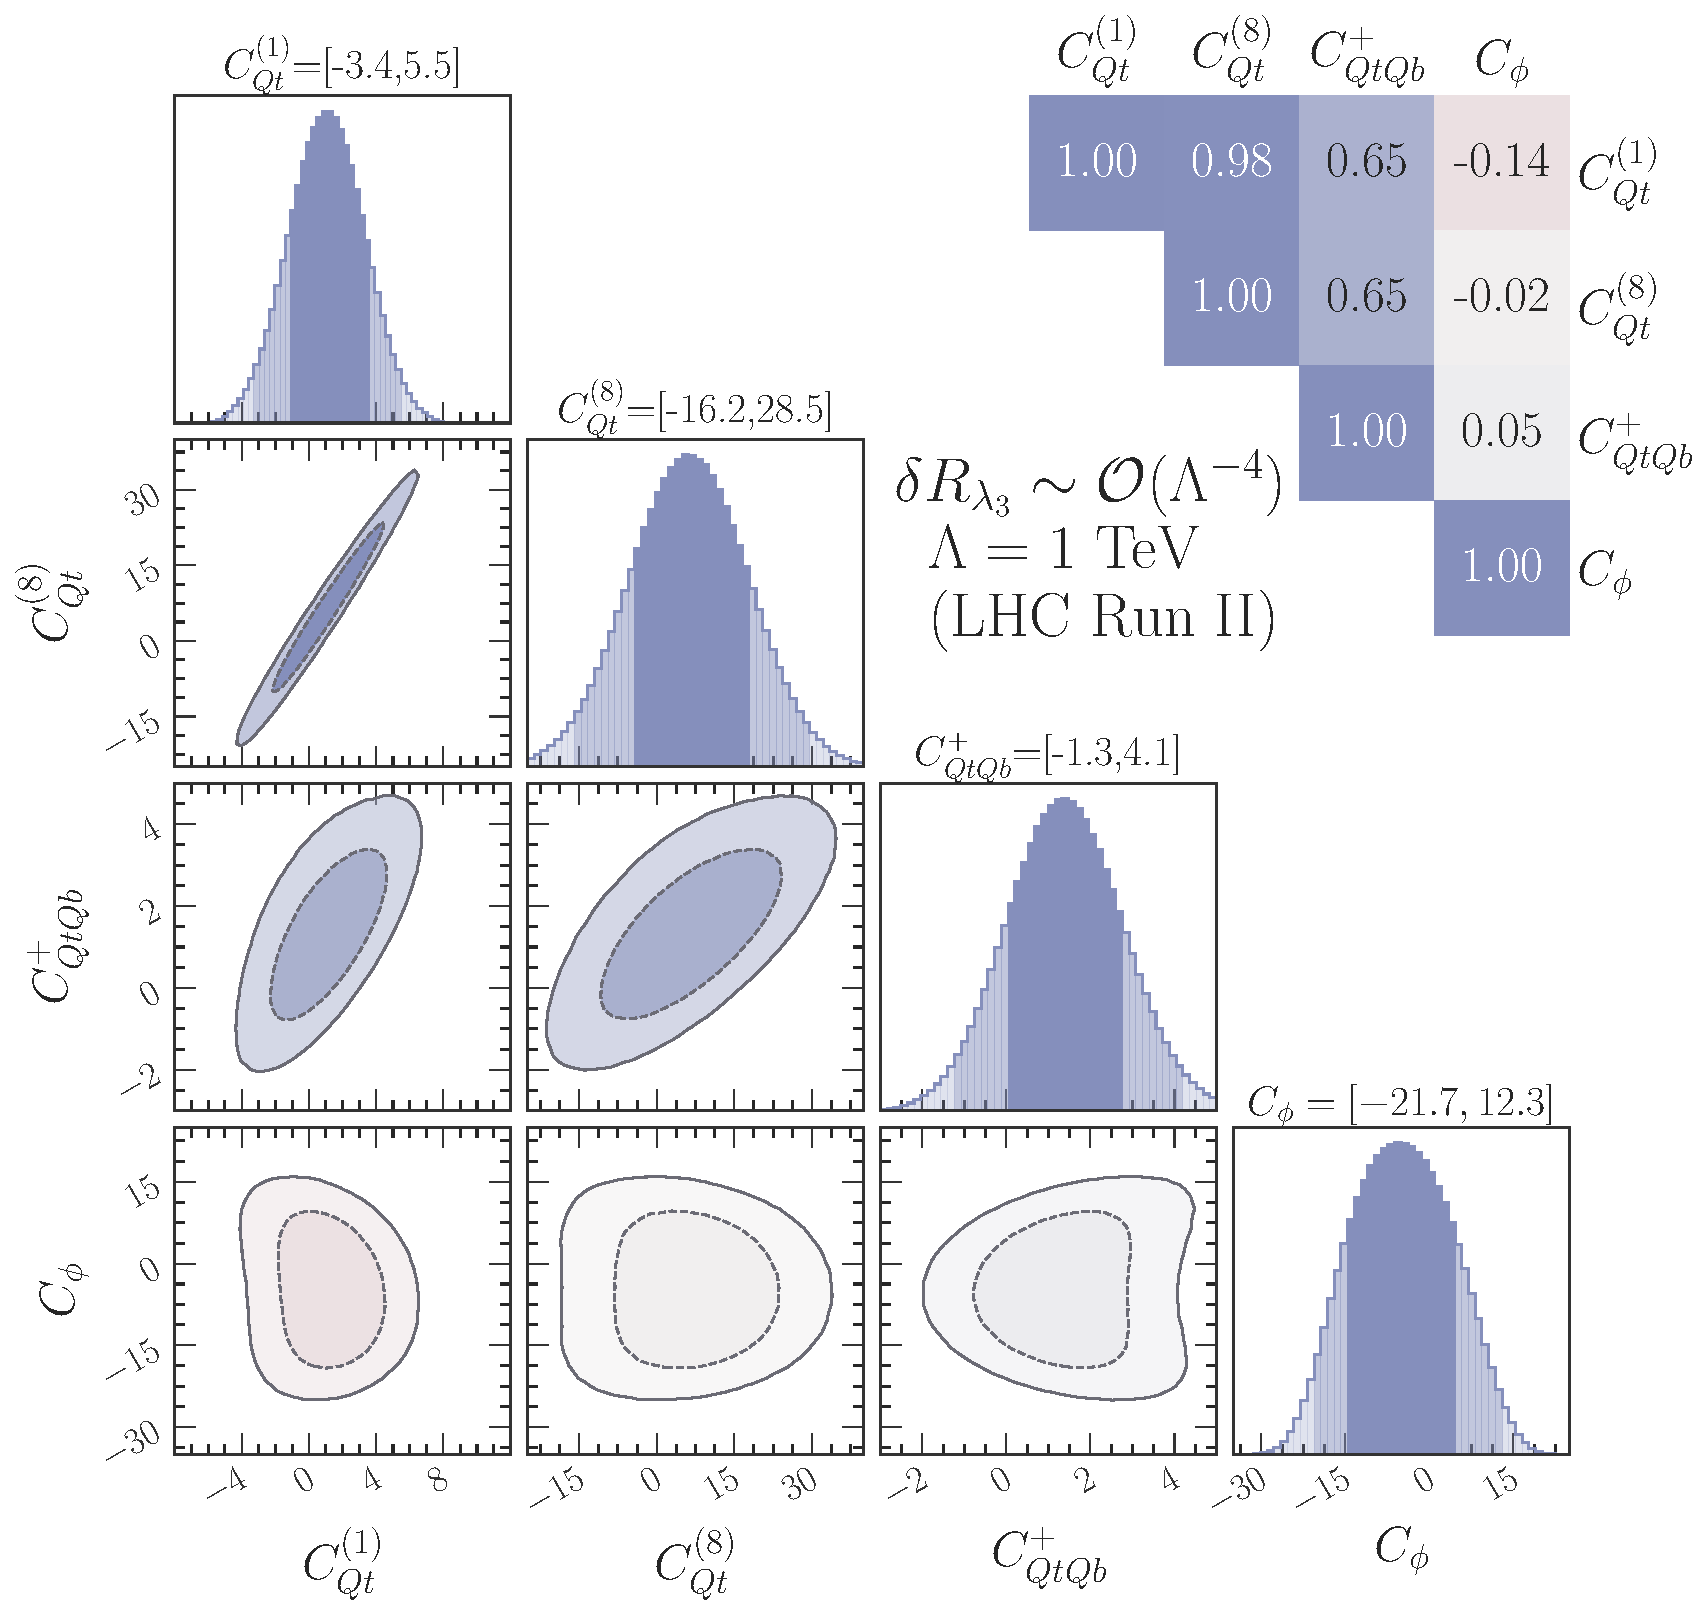
\includegraphics[width=.6\linewidth]{fig/4param_fit_LHC_RunII_l3Q_rge}
			%	\vspace{-.5cm}
		\end{center}
		\caption{The marginalised 68\% and 95\% Highest density posterior contours for the four-parameter fits including the different four-quark Wilson coefficients and $C_\phi$. The numbers above the plots show the 95\% CI bounds while the correlations are given on the top-right side. The correlation between each pair of the Wilson coefficients is highlighted as a heatmap.
			The upper panel shows the fit including up to $\mathcal{O}(1/\Lambda^2)$ in $\delta R_{\lambda_3}$  while the lower one shows the fit with including also  $\mathcal{O}(1/\Lambda^4)$.  This figure has been published in~\cite{Alasfar:2022zyr}. \label{fig:4param} }
	\end{figure}
	%
	When considering two- or four-parameter fits of $C_\phi$ and the four-heavy-quark Wilson coefficients, we observe non-trivial correlation patterns emerging amongst these coefficients.  \autoref{fig:4param} illustrates these correlation patterns for the four-parameter fit. 
	We observe that the Wilson coefficients $C_{Qt}^{(1),(8) }$ are strongly correlated because, in analogy to $C_{QtQb}^{(1),(8) }$, they only appear in particular linear combination whenever correcting the Yukawa coupling. However,  unlike $C_{QtQb}^{(1),(8) }$, they are not entirely degenerate because the main part of the NLO correction to $t\bar t h$ does not contain the aforementioned linear combination.  The four-parameter fit also reveals that the Wilson coefficients~$C_{Qt}^{(1),(8) }$ have a large correlation with ~$C_{QtQb}^{+}$ because all of the four Wilson coefficients appear in a linear combination in the NLO corrections except for $ h\to b\bar b$ and $ t\bar{t} h$. However, this correlation is not as strong due to the large NLO correction of the Higgs decay $h \to b \bar b$ from ~$C_{QtQb}^{(1),(8) }$. Moreover, the correlation between the four-heavy-quark Wilson coefficients and $C_{\phi}$ depends on the $\delta R_{\lambda_3}$ truncation. 
	
	\subsection{Prospects for HL-LHC}
	\begin{figure}[t!]
		\begin{center}
			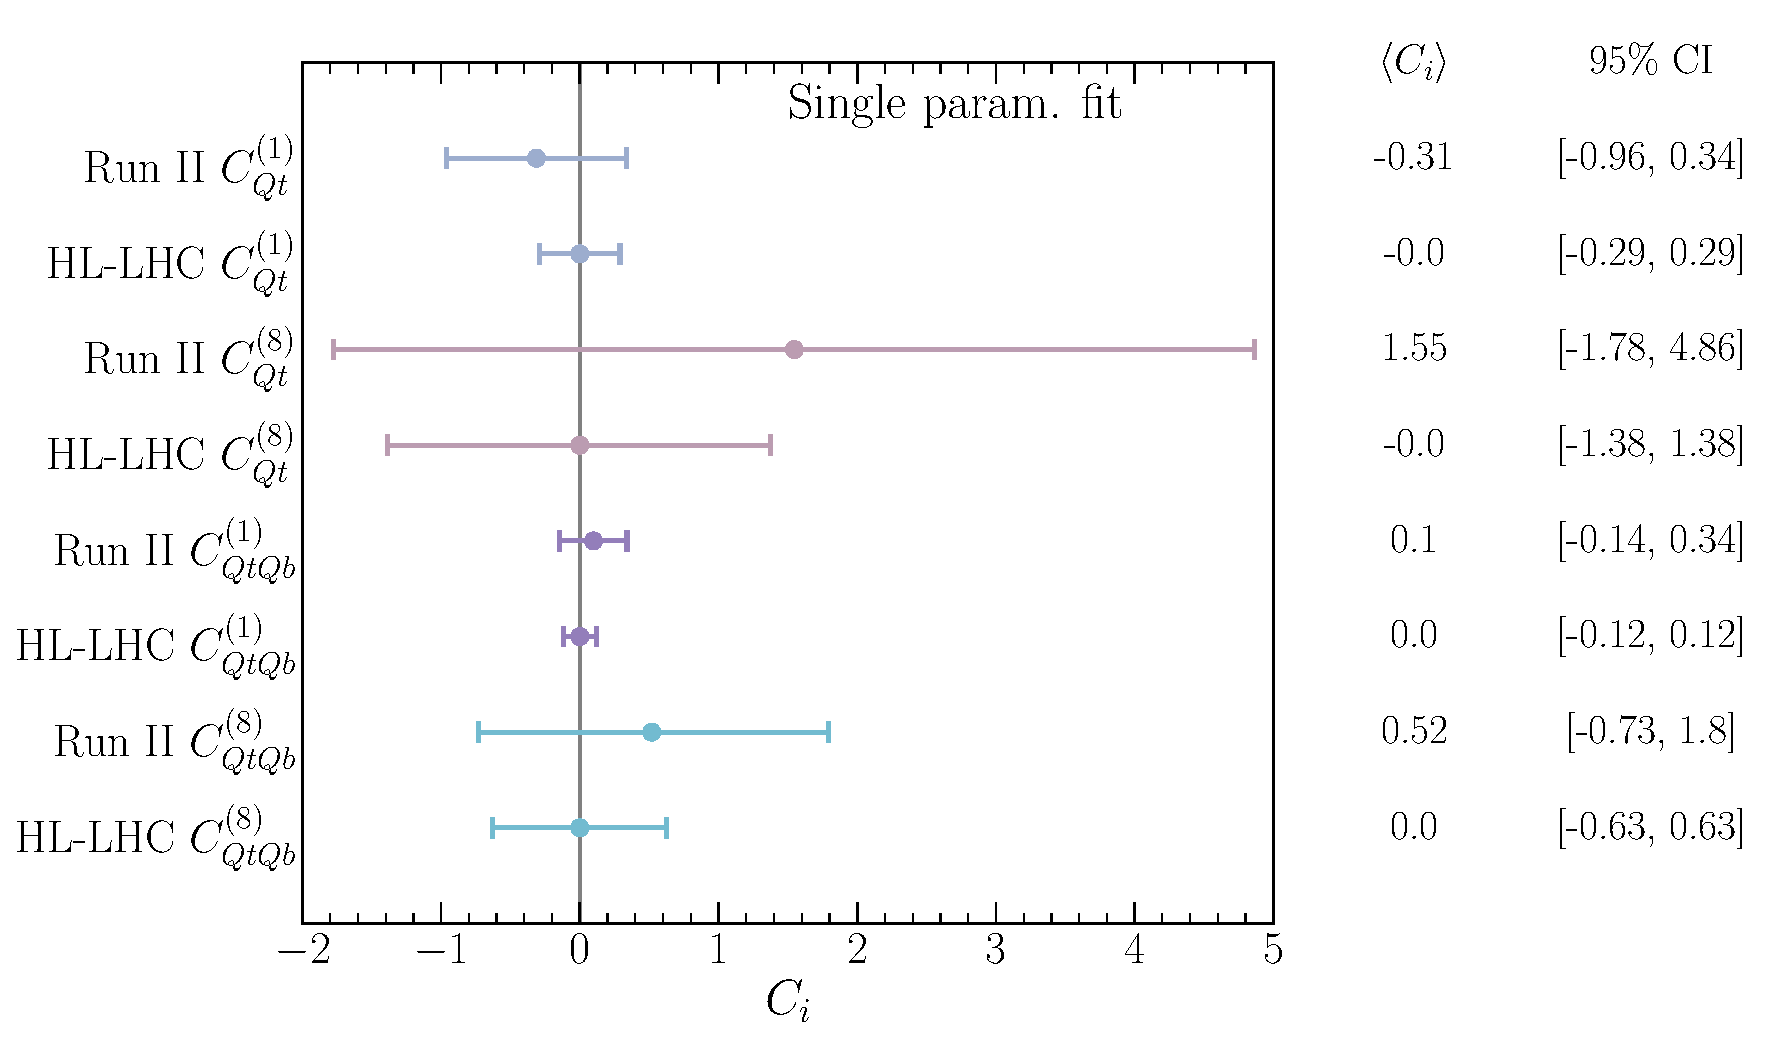
\includegraphics[width=0.75\linewidth]{fig/uebeblick_forest_ci}
		\end{center}
		\caption{ Results of single parameter fit showing the improvement in the constraining power of the HL-LHC over the current bounds from Run-2 data.  This figure has been published in~\cite{Alasfar:2022zyr}. \label{fig:HLLHC} }
	\end{figure}
	
	\begin{figure}
		\begin{center}
			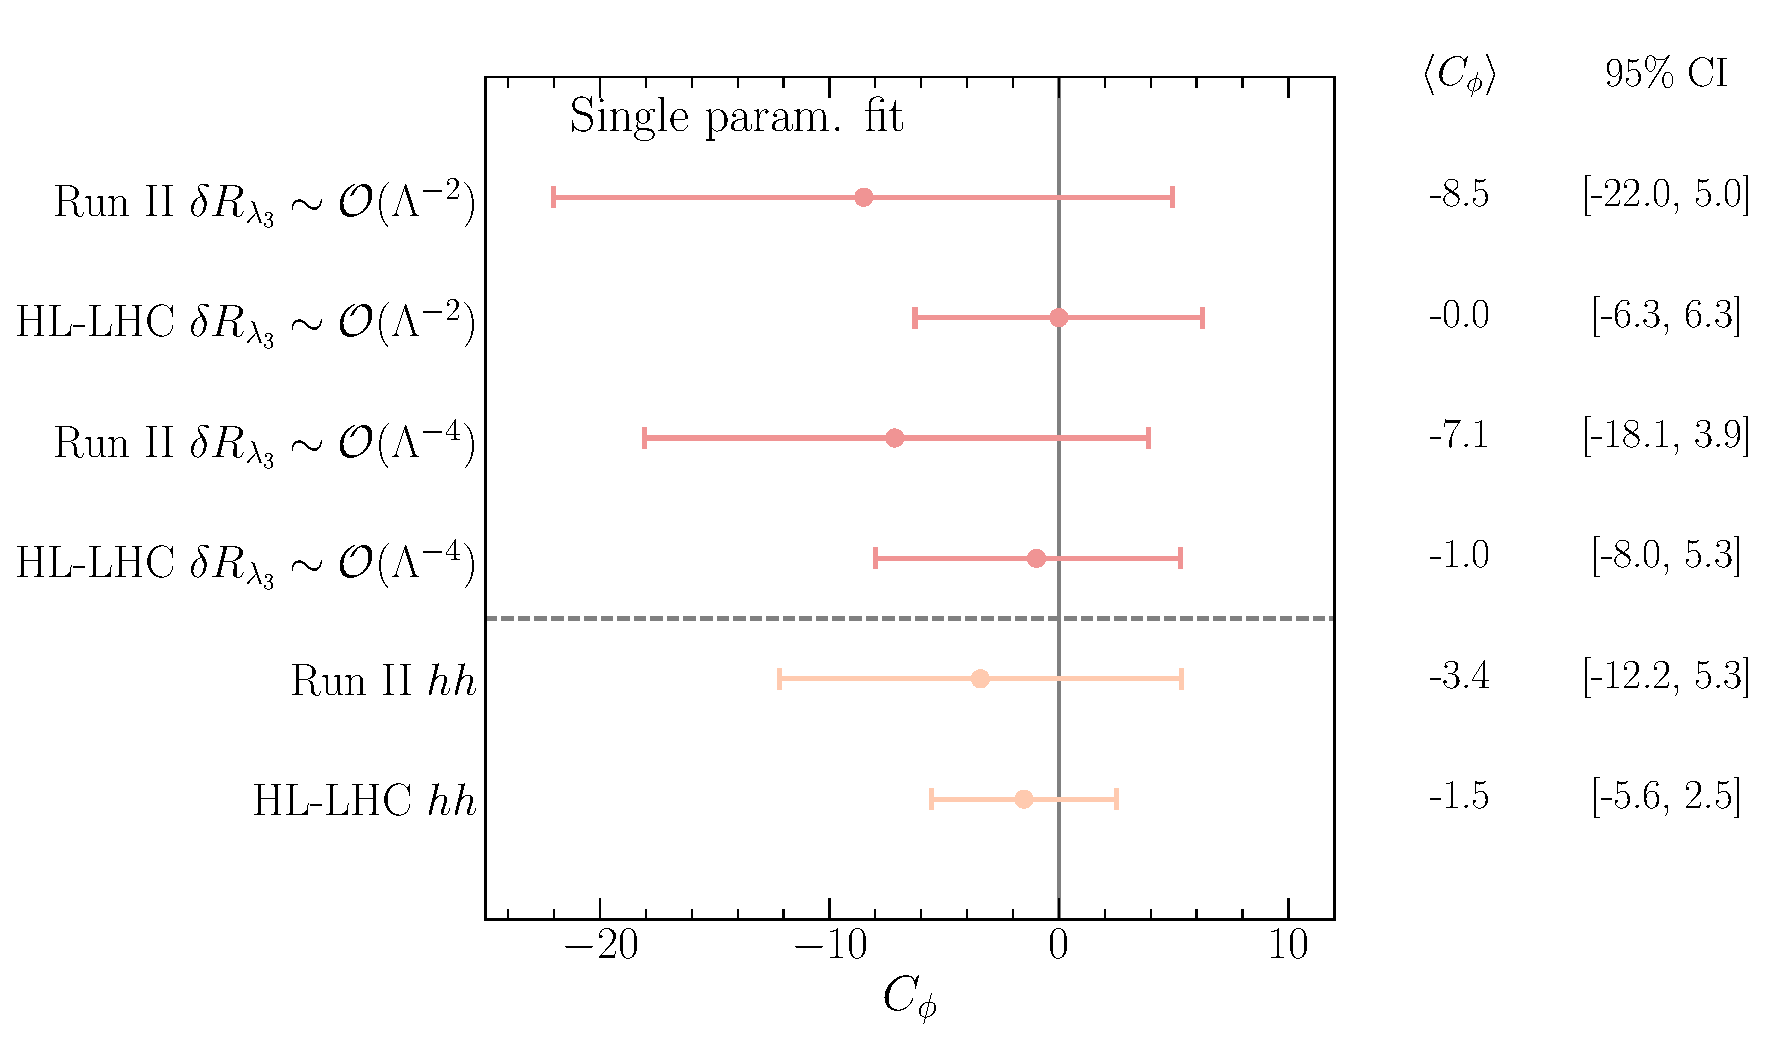
\includegraphics[width=0.75\linewidth]{fig/uebeblick_forest_cphi_singleparam}
		\end{center}
		\caption{A forest plot illustrating the means and 95\% CI's of the posteriors built from the  $C_\phi$  in a single-parameter fit, showing also the differences in including terms of $\mathcal{O}(1/\Lambda^2)$ or up to $\mathcal{O}(1/\Lambda^4)$ in the definition of $\delta R_{\lambda_3}$. For comparison, also the limits and projections from searches for Higgs pair production are shown. This figure has been published in~\cite{Alasfar:2022zyr}.  \label{fig:summcphihl-lhc}  }
	\end{figure}
	Using the CMS Higgs signal strength projections for the HL-LHC in refs.~\cite{CMS-PAS-FTR-18-011,twiki} for a centre-of-mass energy of $\sqrt{s}=14$ TeV and integrated luminosity of $ 3\, \mathrm{ab}^{-1}$, it is possible to repeat the fits done for Run-II.   The projections for the S2 scenario explained in~\cite{Cepeda:2019klc} were used. 
	In \autoref{fig:HLLHC}, I show the comparison between the fit results of Run-II data and the projections for the HL-LHC for single parameter fits. For the operators $\mathcal{O}_{Qt}^{(1),(8)}$ the constraining power of the HL-LHC is roughly a factor two better as the current bounds could be set from single Higgs data, while for the operators $\mathcal{O}_{QtQb}^{(1),(8)}$ the improvement is a little less prominent.
	 In \autoref{fig:summcphihl-lhc}, the limits on $C_{\phi}$ in a single parameter fit for Run-2 and the projections for the HL-LHC are shown.
	including  $\delta R_{\lambda_3}$ up to order $\mathcal{O}(1/\Lambda^2)$ or $\mathcal{O}(1/\Lambda^4)$. While for Run-II data, the inclusion of $\mathcal{O}(1/\Lambda^4)$ made a significant difference; this is less pronounced for the HL-LHC projections. These results are similar to the projections presented in a $\kappa_{\lambda}$ fit in \cite{DiMicco:2019ngk}. 
	The results were also confronted with data from searches for Higgs pair production $139$ fb$^{-1}$ \cite{ATLAS:2021jki}  and HL-LHC projections~\cite{CMS:2018ccd} on Higgs pair production, showing that Higgs pair production would still allow setting firmer limits on $C_{\phi}$. 
	%%%%%%%%%%%%%%%%%%%%%%%%%%%%%%
	\section{Conclusion \label{sec:conclusion4tops}}
	%%%%%%%%%%%%%%%%%%%%%%%%%%%%%%
	This chapter calculates the NLO corrections emanating from the SMEFT four-heavy-quark operators to single-Higgs rates. We have seen that both four-fermion operators' classes involving homogenous and heterogeneous chirality structures contribute to Higgs rates at NLO. Though, the operators with heterogeneous chirality structures have more sizeable effects as they would contribute to $h f\bar f$ vertex correction and quark mass renormalisation in SMEFT. Therefore, the appear in more channels compared to the operators baring homogenous chirality structures. The results of these calculations were utilised in fits on the Wilson coefficients associated with these operators using single-Higgs data. The operators with the same chirality structure are not constrained strongly by these fits, and hence their results were not included. This applies to the operators that contribute only via beauty-quark loops, like $\mathcal{O}_{Qb}^{(1),(8)}$. \\ Two processes stood out in this calculation in terms of their sensitivity to these operators. The first process is the decay of the Higgs to beauty quarks, which had a strong sensitivity to $\mathcal{O}_{QtQb}^{(1),(8)}$ operators, The second process is the associated production of the Higgs with top pair~$t \bar th$ having large finite corrections coming from $\mathcal{O}_{Qt}^{(1),(8)}$. Furthermore, these corrections depend on the colour factor and thus break the degeneracy between the singlet and octet operators. \\
	Bayesian analysis combining the four-fermion operators with the SMEFT operator modifying the Higgs self-coupling $C_\phi$ has been performed and motivated by the fact that both operators are weakly constrained and only appear at NLO in single-Higgs rates. The fit results showed that the constraints on $C_\phi$ from single Higgs data would become significantly diluted compared to the fits performed with this operator alone, or even with ones that enter at LO~\cite{Gorbahn:2016uoy, Degrassi:2016wml, Bizon:2016wgr, Maltoni:2017ims, Degrassi:2021uik}. This is due to the strong correlation between $C_\phi$ and the four-fermion operators considered in this study. On the other hand, the fits yielded stronger bounds on the four-heavy-quark operators than those obtained from top-quark data \cite{Ethier:2021bye, Hartland:2019bjb}. Comparable bounds can also be seen when EWPO data is considered for their fit, cf.~\cite{Dawson:2022bxd}. Similarly to single-Higgs processes, EWPO are modfied by these operators at NLO, as well. Additionally, the authors of ref.~\cite{Silvestrini:2018dos} have shown that these operators could also be constrained from flavour observables involving $\Delta F=2$, in particular~$B_s -\bar{B}_s$ mixing. However, these bounds depend on the flavour ansatz of the NP and hence are not entirely model-independent. \\ The results of these calculations and consequent fits further emphasise the interconnectivity of SMEFT operators and experimental observables, which was discussed in\autoref{chap: HiggsEFT}. \\
	Then remains the question: \textit{How this interconnectivity would manifest in an NP model ?}. Remarkably, one might wonder if the strong correlation between these four-fermion operators and $\mathcal{O}_\phi$ could appear in a UV complete model. In fact, large effective couplings involving four top quarks are expected in many NP models, for example, partial compositeness~\cite{Banelli:2020iau}. These models would also generate sizeable modifications to the Higgs self-interaction. Similar effects could be obtained from models containing new scalars, such as an additional Higgs doublet~$\varphi\sim (1,2)_{\frac 12}$, or other scalars with non-singlet representation under $SU(3)_c$ like~ $(6,1)_{\frac 1 3}$ and $(8,2)_{\frac 1 2}$. For further details on these models and their matching, see~\cite{deBlas:2017xtg}; for the NLO matching to SMEFT, see \cite{Anisha:2021hgc}. 